%%%%%%%%%%%%%%%%%%%%%%%%%%%%%%%%%%%%%%%%%
\documentclass[a5paper,doc,10pt,noapacite]{apa6}
%----------------------------------------------------------------------------------------
%	Paquetes y configuraciones
%----------------------------------------------------------------------------------------
\usepackage[hidelinks]{hyperref}
\usepackage[unnumberedbib,notocbib]{apacite}
%\usepackage{chapterbib} % bibunits???
\usepackage{bibunits}

\usepackage{amsfonts} 
\usepackage{amsmath}
\usepackage{amssymb,amsthm}
\usepackage{enumerate}
\usepackage{enumitem}
\usepackage[utf8]{inputenc}
\usepackage[T1]{fontenc}
\usepackage[spanish,es-nolayout,es-nodecimaldot,es-tabla]{babel}
\geometry{top=2.5cm, bottom=2.5cm, left=2.5cm, right=2.5cm, headheight=1.8cm,headsep=.5cm,footskip=1.3cm}

\usepackage{url}
\def\UrlBreaks{\do\/\do-}
\def\pnorm||#1||_#2,#3{||#1||_{L^{#2}(#3)}}
\usepackage{multirow}
\usepackage{multicol}
\usepackage{enumitem}
\usepackage{nicefrac}
\usepackage{graphicx}
\usepackage{stmaryrd}
\usepackage{dsfont}
\usepackage{bropd}
\usepackage{easybmat}
\usepackage[table,xcdraw]{xcolor}
\usepackage{longtable} 
\usepackage{setspace}
\usepackage{comment}
\usepackage{mathpazo}
\usepackage{array}
\usepackage{wrapfig}
\usepackage{ragged2e}
\usepackage{hyperref}
\usepackage{bigstrut}
\usepackage{tabularx}

\usepackage{sectsty}
\sectionfont{\centering\fontsize{13}{15}\selectfont}

\subsectionfont{\centering\fontsize{10}{10}\selectfont\scshape}
\subsectionfont{\fontsize{9.5}{10}\selectfont}

\subsubsectionfont{\centering\fontsize{9}{10}\selectfont}
\subparagraphfont{\centering\fontsize{8.5}{10}\selectfont}

\usepackage[titles]{tocloft}
\usepackage{textcomp }

\usepackage{csquotes}
\usepackage{floatrow}

\newfloatcommand{capbtabbox}{table}[][\FBwidth]

% Comandos
\newcommand{\bull}{\textbullet \ }
\newcommand{\EPN}{Escuela Politécnica Nacional}
\newcommand{\Modemat}{Centro de Modelización Matemática, ModeMat-EPN}%{ModeMat -- Escuela Politécnica Nacional}
\newcommand{\Modematb}{Centro de Modelización Matemática, ModeMat-EPN}

\newcommand{\R}{\mathbb{R}}
\newcommand{\N}{\mathbb{N}}
\newcommand{\Z}{\mathbb{Z}}
\newcommand{\C}{\mathbb{C}}
\newcommand{\dsum}{\displaystyle \sum}
\newcommand{\yds}{\qquad\text{y}\qquad}
\newcommand{\tendsto}[1][ ]{\stackrel{ #1 }{\longrightarrow}}
\newcommand{\subKeps}[2][k]{#2_{#1,\varepsilon}}
\DeclareMathOperator{\Dom}{Dom}
\DeclareMathOperator{\Ran}{Ran}
\DeclareMathOperator{\inv}{inv}
\DeclareMathOperator{\Res}{Res}
\DeclareMathOperator{\Ind}{Ind}
\DeclareMathOperator{\im}{Im}
\DeclareMathOperator{\CEiP}{CEiP}
\DeclareMathOperator{\dive}{div}
\DeclareMathOperator{\Esp}{E}
\DeclareMathOperator{\Var}{V}
\DeclareMathOperator{\cov}{cov}
\DeclareMathOperator{\Normal}{\mathcal{N}}
\DeclareMathOperator{\sen}{sen}

\newtheorem{definicion}{Definición}
\newtheorem{proposicion}{Proposición}
\newtheorem{teorema}{Teorema}
\newtheorem{observ}{Observación}
\newtheorem{ejem}{Ejemplo}
\newtheorem*{objetivo}{Objetivo}
\newtheorem*{objetivos}{Objetivos}


%%%mycolors
\definecolor{palegreen}{rgb}{0.6, 0.98, 0.6}
\definecolor{paleblue}{rgb}{0.69, 0.93, 0.93}
\definecolor{pastelyellow}{rgb}{0.99, 0.99, 0.59}
\definecolor{pastelgray}{rgb}{0.81, 0.81, 0.77}
\definecolor{pastelgreen}{rgb}{0.47, 0.87, 0.47}
\definecolor{pastelblue}{rgb}{0.68, 0.78, 0.81}

\newcommand{\vsb}{\vspace{0.75\baselineskip}}
\newcommand{\Speaker}[4]{\vsb #1 \\ \emph{#2} \\ \textsc{#3}\\ \texttt{#4}}


\setlength{\parindent}{0pt}
\linespread{1.5}

\usepackage[10pt]{moresize}

\usepackage{xspace}
\makeatletter
\DeclareRobustCommand{\maybefakesc}[1]{%
  \ifnum\pdfstrcmp{\f@series}{\bfdefault}=\z@
    {\fontsize{\dimexpr0.8\dimexpr\f@size pt\relax}{0}\selectfont\uppercase{#1}}%
  \else
    \textsc{#1}%
  \fi
}
\newcommand\AM{\,\maybefakesc{am}\xspace}
\newcommand\PM{\,\maybefakesc{pm}\xspace}
\makeatother


%---------------------------------------- Autoría ---------------------------------------- %
\title{Plantilla LAWOC}
\author{Andy}
\shorttitle{}
\date{\today}

%---------------------------------------- Citas  ------------------------------------------ %
\renewcommand\bibliographytypesize{\footnotesize}


%------------------------------------- Abstracts ---------------------------------------- %
\newcommand{\pto}{$\cdot$ }

% AbstractA no contiene elementos bibliográficos
\newcommand{\AbstractA}[6]{%
	\addcontentsline{toc}{subsection}{#1 \footnotesize(\emph{#2})}
	\begin{center}
		\bf\scshape#1
	\end{center}
	%\subsection{#1}
	\vspace{-0.85\baselineskip}
	%
	%
	\begin{center}
		{\scriptsize% 
			  #2		\bull			% Autor
		\textsf{#3}		\bull			% Institución
		\texttt{#4}		\\[-1em]		% Correo
		\emph{#5} }				%.Área
	\end{center}
	\vspace{-0.5\baselineskip}
	\begin{spacing}{1.2}
		\footnotesize
		\hspace{15.0pt}
		#6	
	\end{spacing}
	\vspace{1\baselineskip}
}

% AbstractCA no contiene elementos bibliográficos
\newcommand{\AbstractCA}[7]{%
	\addcontentsline{toc}{subsection}{#1 \footnotesize(\emph{#2})}
	\begin{center}
		\bf\scshape#1
	\end{center}
	%\subsection{#1}
	\vspace{-0.85\baselineskip}
	%
	%
	\begin{center}
		{\scriptsize% 
			  #2					% Autor
			  #3		\bull			% Co-autores
		\textsf{#4}		\bull			% Institución
		\texttt{#5}		\\[-1em]		% Correo
		\emph{#6} }				%.Área
	\end{center}
	\vspace{-0.5\baselineskip}
	\begin{spacing}{1.2}
		\footnotesize
		\hspace{15.0pt}
		#7	
	\end{spacing}
	\vspace{1\baselineskip}
}

% Abstract B sí contiene bibliografía
\newcommand{\AbstractB}[6]{%
	\addcontentsline{toc}{subsection}{#1 \footnotesize(\emph{#2})}
	\begin{center}
		\bf\scshape#1
	\end{center}
	%\subsection{#1}
	\vspace{-0.85\baselineskip}
	%
	\begin{center}
		{\scriptsize% 
			  #2		\bull			% Autor
		\textsf{#3}		\bull			% Institución
		\texttt{#4}		\\[-1em]		% Correo
		\emph{#5} }				%.Área
	\end{center}
	\vspace{-0.5\baselineskip}
	\begin{spacing}{1.2}
		\begin{bibunit}
			\footnotesize
			\hspace{15.0pt}
			#6
			\addtocontents{toc}{\protect\setcounter{tocdepth}{-1}}	
			\putbib
			\addtocontents{toc}{\protect\setcounter{tocdepth}{2}}
		\end{bibunit}\vspace{0.5\baselineskip}
	\end{spacing}
}

% Abstract B sí contiene bibliografía
\newcommand{\AbstractCB}[7]{%
	\addcontentsline{toc}{subsection}{#1 \footnotesize(\emph{#2})}
	\begin{center}
		\bf\scshape#1
	\end{center}
	%\subsection{#1}
	\vspace{-0.85\baselineskip}
	%
	\begin{center}
		{\scriptsize% 
			  #2					% Autor
			  #3		\bull			% Co-autores
		\textsf{#4}		\bull			% Institución
		\texttt{#5}		\\[-1em]		% Correo
		\emph{#6} }				%.Área
	\end{center}
	\vspace{-0.5\baselineskip}
	\begin{spacing}{1.2}
		\begin{bibunit}
			\footnotesize
			\hspace{15.0pt}
			#7
			\addtocontents{toc}{\protect\setcounter{tocdepth}{-1}}	
			\putbib
			\addtocontents{toc}{\protect\setcounter{tocdepth}{2}}
		\end{bibunit}\vspace{0.5\baselineskip}
	\end{spacing}
}

% Curso tutorial
\newcommand{\Tutorial}[5]{%
\addcontentsline{toc}{section}{#1 \footnotesize(\emph{#2})}
	\begin{center}
		\bf\scshape #1
	\end{center}
	%\subsection{#1}
	\vspace{-0.85\baselineskip}
	%
	\begin{center}
		{\scriptsize% 
			  #2		\bull			% Autor
		\textsf{#3}		\bull			% Institución
		\texttt{#4}		\\[-1em]		% Correo 
		}
	\end{center}
	\vspace{-0.5\baselineskip}
	%
	
	\begin{spacing}{1}
		\begin{bibunit}
			\footnotesize
			#5
			%\addtocontents{toc}{\protect\setcounter{tocdepth}{-1}}	
			\putbib
			%\addtocontents{toc}{\protect\setcounter{tocdepth}{2}}
		\end{bibunit}\vspace{0.5\baselineskip}
	\end{spacing}
}

%------------------------------------- Información turística ---------------------------------------- %

\newcommand{\InfoTour}[6]{%
\qquad \textbf{\textsc{#1:}}%
#2

\qquad
\begin{tabular}{p{1.5cm} p{7cm}}
	Hours 	& #3
	\\
	Location	& #4
	\\
	Prices	& #5
    \\
    Website & {\scriptsize\texttt{#6}}
\end{tabular}
\vspace{\baselineskip}
}

\newcommand{\InfoTourb}[2]{%
\qquad \textbf{\textsc{#1:}}%
#2
\vspace{\baselineskip}
}

\newcommand{\InfoTourc}[6]{%
\quad \emph{#1:}%
#2

\quad
\begin{tabular}{p{1.5cm} p{7cm}}
	Hours 	& #3
	\\
	Location	& #4
	\\
	Prices	& #5
    \\
    Website & {\scriptsize\texttt{#6}}
\end{tabular}
\vspace{\baselineskip}
}

\newcommand{\Rest}[3]{%
\begin{tabular}{>{\bf\scshape}p{3.5cm} >{\em\centering\arraybackslash}p{2cm}    >
{\raggedleft\arraybackslash}p{4cm}}
	#1  & #2 & #3
\end{tabular}
\vspace{0.4\baselineskip}
}

\renewcommand{\BCBT}{}

% -------------- Pseudo definición fuera de entorno que no me gustó pero toca respetar las malas costumbres de algún modo

\newcommand{\neodefi}[1]{%
	\vspace{1\baselineskip}
	\textbf{\small#1} \newline
}

%--------------------------------------------------------------------------------------------------------------------------------------
%----------------------------------------------------------------------------------------
%------------------------------------------
\begin{document}
\pagestyle{empty}
\pagenumbering{gobble} 
%%%%%%%%%%%%%%%%%%%%%%%%
%      Título
%%%%%%%%%%%%%%%%%%%%%%%%
\newgeometry{top=4cm, bottom=2cm, left=2.5cm, right=2.5cm}
{
	\HUGE
	{\bf\textsc{XVI \\[0.5cm] Encuentro  \\[0.5cm] de Matemática \\[0.5cm] y sus Aplicaciones \\[0.5cm] }}
	\\[1cm]
	\large
	
	\vspace{-1.75cm}
	\begin{center}
		
		\textsc{Introducción a la teoría de estabilidad: sistemas de ecuaciones diferenciales ordinarias}
		
		\vspace{1\baselineskip}
		
		Ménthor Urvina
		\\
		
		\normalsize
		\EPN, Ecuador
	\end{center}
}

\vspace{1.75cm}
\begin{center}
	
\includegraphics[height=2.45cm]{Logos/DM-EPN}
\end{center}

%\clearpage\null\newpage
%%%%%%%%%%%%%%%%%%%%%%%%
%      Datos de edición
%%%%%%%%%%%%%%%%%%%%%%%%
\newpage
\newgeometry{top=4cm, bottom=2cm, left=2cm, right=2cm}
\mbox{}
\vfill
{
\footnotesize
\textsc{XVI Encuentro de Matemática y sus Aplicaciones}

22 -- 26 de octubre de 2018

Quito, Ecuador

%
\vspace{1\baselineskip}
\emph{Comité Organizador}
\begin{spacing}{1.2}
\scriptsize
	Polo Vacas		\bull Paúl Acevedo	\bull Adriana Uquillas	
	
	\emph{\EPN}
\end{spacing}

%
\vspace{1\baselineskip}
\emph{Comité Científico}
\begin{spacing}{1.2}
\scriptsize
	Marco Calahorrano Recalde	--	\emph{\EPN, ECUADOR} 		\bull 
	Diego Chamorro			-- 	\emph{Université d'Évry, FRANCIA} \bull
	Juan Carlos De los Reyes		-- 	\emph{\EPN, ECUADOR} \bull
	Luis Horna				--	\emph{\EPN, ECUADOR} \bull
	Luis Miguel Torres			--	\emph{\EPN, ECUADOR} 
%		
\end{spacing}

%
\vspace{1\baselineskip}
\emph{De esta edición}
\begin{spacing}{1.2}
\scriptsize
	\emph{Editor:} 	Andrés Miniguano Trujillo 	--	\emph{\Modemat, ECUADOR}
	
	\emph{Asistentes:} Eduardo Arias, Erika Ludeña -- \emph{\EPN, ECUADOR}
	
	\emph{Diseño arte:} Julio Erazo -- \emph{\EPN, ECUADOR}
	
	\emph{Adaptación de portada:} Belén Santacruz Reyes
%		
\end{spacing}

%
\vspace{1\baselineskip}
\emph{Auspiciantes}
\begin{spacing}{1.2}
\scriptsize
	Sociedad Ecuatoriana de Matemática \emph{(SEdeM)}				\bull
	\Modemat													\bull
	Actuaria: Asesoramiento Estratégico
\end{spacing}

%
\vspace{1\baselineskip}
\emph{Con el apoyo de}
\begin{spacing}{1.2}
\scriptsize
	Escuela Politécnica Nacional \emph{(EPN)}						\bull
	Departamento de Matemática EPN
\end{spacing}


% Logos
\vspace{1.5\baselineskip}
\begin{center}
	
\includegraphics[height=1cm]{Logos/SEdeM}
	\qquad\quad
	
\includegraphics[height=1cm]{Logos/ModeMat}
	\qquad\quad
	
\includegraphics[width=2.5cm]{Logos/logo-actuaria}			%*
	\qquad\quad
	
\includegraphics[height=1cm]{Logos/EPN}
	\qquad\quad
	
\includegraphics[height=1cm]{Logos/DM-EPN}
\end{center}

% Contenidos
\newpage
\pagestyle{empty}
\pagenumbering{arabic}
\setcounter{page}{0}
\newgeometry{top=2cm, bottom=2cm, left=2cm, right=2cm, headheight=1.8cm,headsep=.5cm,footskip=1.3cm}
%\normalsize
\small
\tableofcontents



%----------------------------------------------------------------------------------------
\newpage
\pagestyle{plain}
%%%%%%%%%%%%%%%%%%%%%%%%
%%%%%%%%%%%%%%%%%%%%%%%%
% \section{Program}
% \normalsize
% adad
%que no pongamos el programa


%----------------------------------------------------------------------------------------
\newpage
%%%%%%%%%%%%%%%%%%%%%%%%
%%%%%%%%%%%%%%%%%%%%%%%%
\newgeometry{top=2cm, bottom=2cm, left=1.75cm, right=1.75cm, headheight=1.8cm,headsep=.5cm,footskip=1.3cm}

\begin{comment}
\section{Presentación}
\footnotesize

The VI Latin American Workshop on Optimization and Control will take place in Quito, Ecuador, September 3 - 7, 2018. The event is organized on a biennial basis with the main goal of boosting the development and interaction between these two scientific disciplines in Latin America. Therefore, the workshop gathers outstanding senior and junior researchers, postdoctoral fellows, and graduate students working in these fields.

\vspace{0.5\baselineskip}
The event focuses, among others, on the following topics:
\begin{APAitemize}
	\item Optimal Control
    \item Inverse Problems
    \item Nonsmooth Optimization
    \item Control of Partial Differential Equations
\end{APAitemize}

\vspace{0.5\baselineskip}
The first edition of this event was held in Quito, Ecuador, in July 2008, based on an initiative of researchers from Escuela Politécnica Nacional, Ecuador, and Universidad Nacional de Rosario, Argentina. The second edition was held in 2010 in Rosario, Argentina, with the same organizers. Subsequently, a third edition took place in 2012 in Valparaiso, Chile; a fourth edition in 2014 in Lima, Peru; and a fifth edition was held in 2016 in Tandil, Argentina.

\vspace{0.5\baselineskip}
An additional goal of the workshop is to increase of visibility of Optimization and Control among advanced undergraduate students (in Mathematics, Computer Science, Engineering, Physics, Economics and others).
\end{comment}

%----------------------------------------------------------------------------------------
\newpage
%%%%%%%%%%%%%%%%%%%%%%%%
%%%%%%%%%%%%%%%%%%%%%%%%
\newgeometry{top=2cm, bottom=2cm, left=1.75cm, right=1.75cm, headheight=1.8cm,headsep=.5cm,footskip=1.3cm}

\bibliographyunit[\subsection]
\bibliography*{citas.bib}
\bibliographystyle*{apacite}
\bibliographyunit
\renewcommand{\refname}{\small Referencias}



%----------------------------------------------------------------------------------------


%%%%%%%%%%%%%%%%%%%%%%%%
%%%%%%%%%%%%%%%%%%%%%%%%
%
\footnotesize
\normalsize

\newgeometry{top=2cm, bottom=2cm, left=2cm, right=2cm, headheight=1.8cm,headsep=.5cm,footskip=1.3cm}


% ------------------ Menthor ------------------%
\Tutorial{Introducción a la teoría de estabilidad: sistemas de ecuaciones diferenciales ordinarias}{Ménthor Urvina}{\EPN, Ecuador}{menthor.urvina@epn.edu.ec}{

\vspace{1\baselineskip}\setcounter{figure}{0} \setcounter{teorema}{0} \setcounter{definicion}{0} \setcounter{proposicion}{0}
\setcounter{ejem}{0} \setcounter{observ}{0}

En el documento se presentan las principales definiciones usadas en estabilidad: sistemas autónomos, plano de fase, puntos críticos, estabilidad; así como los principales resultados para determinar la naturaleza de los puntos críticos y su estabilidad.

\subsection{Sistemas autónomos, el plano de fase}

A menudo sucede que muchas ecuaciones diferenciales ordinarias (o sistemas de ecuaciones diferenciales ordinarias) no pueden resolverse analíticamente en forma explícita, pero se puede analizar el comportamiento cualitativo de sus soluciones, sin el conocimiento explícito de ellas.

En lo que sigue se estudian sistemas de ecuaciones diferenciales ordinarias de la forma:
\begin{equation}\label{m-1}
	\begin{cases}
		\dfrac{dx}{dt}=F(x,y) ,\vspace{0.3em}
		\\
		\dfrac{dy}{dt}=G(x,y),
	\end{cases}
\end{equation}
donde \(F=F(x,y)\), \(G=G(x,y)\) y sus derivadas parciales son continuas en todo el plano.

EL sistema \eqref{m-1} en el que la variable  independiente \(t\) no aparece explícitamente en \(F\) y \(G\) se llama \emph{\textbf{autónomo}}.

Por el teorema de existencia y unicidad, se tiene que para cualquier \(t_0\in\R\) y \((x_0,y_0)\in\R^2\), el sistema anterior tiene una solución única: 
\begin{equation}\label{m-2}
	\begin{cases}
		x=x(t),	
		 \\
		y = y(t);
	\end{cases}
\end{equation}
que satisface la condición inicial: 
\[
	\begin{cases}
		x(t_0)=x_0,
		 \\
		y(t_0) = y_0.
	\end{cases}
\]

La solución del sistema \(\begin{cases}	x=x(t),	\\		y = y(t),	\end{cases}\) \hspace{-1em} corresponde a la representación paramétrica de una curva en el plano \(xy\), al cual se le llama plano de fase y la curva solución se denomina trayectoria del sistema, y se denota con \(\Gamma=\Gamma(x,y)=\Gamma\big(x(t),y(t)\big)\). La familia de trayectorias representadas en el plano de fase se denomina el retrato de fase.
	
\begin{observ}
	Si \eqref{m-2} es la solución de \eqref{m-1} se puede mostrar que:
	\begin{equation}\label{m-2}
	\begin{cases}
		x=x(t+c),	
		 \\
		y = y(t+c),
	\end{cases}
	\end{equation}
	también es solución del sistema, para cualquier constante \(c\), luego:
	\[
	\Gamma=\Gamma(x,y)=\Gamma\big(x(t+c),y(t+c)\big).
	\]
	Es decir cada trayectoria viene representada por muchas soluciones que difieren entre sí por una traslación del parámetro. Como el problema de valor inicial tiene solución, entonces por cada punto \((x_0,y_0)\) pasa una sola trayectoria, esto significa que las trayectorias no se intersecan.
\end{observ}

\begin{observ}\quad
	\begin{APAenumerate}
		\item La dirección \(t\) creciente a lo largo de la trayectoria dada es la misma para todas las soluciones que representa a esa trayectoria. Una trayectoria \(\Gamma=\Gamma(x,y)\)  es por tanto una curva dirigida, en los gráficos se utilizan flechas para indicar la dirección de \(t\) creciente sobre las trayectorias.
		
		\item Para los sistemas
		\[
			\begin{cases}
			x' = F(x,y),
			 \\
			y' = G(x,y),
			\end{cases}
			\yds
			\begin{cases}
			x' = -F(x,y),
			 \\
			y' = -G(x,y),
			\end{cases}
		\]
		Los diagramas de fase son los mismos, excepto que la orientación en las trayectorias se invierte.


		\item Para el punto \((x_0,y_0)\) tal que
		\(
			\begin{cases}
			x' = F(x_0,y_0)=0,
			 \\
			y' = G(x_0,y_0)=0,
			\end{cases}
		\)\hspace{-1em}
		se cumple que 
		\(
			\begin{cases}
			x(t) = x_0,
			 \\
			y(t) = y_0,
			\end{cases}
		\)\hspace{-1em}
		es también solución, pero no es una  trayectoria.
		
		
	\end{APAenumerate}
\end{observ}

De las observaciones anteriores se concluye que las trayectorias cubren todo el plano de fase y no se intersecan entre sí, la única excepción ocurre en los puntos \((x_0,y_0)\) donde \(F\) y \(G\) son cero.



\subsubsection{Punto crítico}

\begin{definicion}
	Al punto \((x_0,y_0)\) que satisface \(\begin{cases}
			F(x_0,y_0)=0,
			 \\
			G(x_0,y_0)=0,
			\end{cases}
		\)\hspace{-1em}, se lo denomina \textbf{\emph{punto crítico}} del sistema.
\end{definicion}

\begin{observ}
	En los puntos críticos, la única solución del sistema es la solución constante \(x(t)=x_0\), \(y(t)=y_0\) y no define una trayectoria, así que por un punto crítico no pasa ninguna trayectoria.
	
	Se supondrá que todo punto crítico \((x_0,y_0)\) es \emph{\textbf{aislado}}, es decir, existe un círculo centrado en \((x_0,y_0)\)  que no contiene otro punto crítico.
\end{observ}

\begin{ejem}
	La ecuación del movimiento de un péndulo amortiguado es:
	\[
	\dfrac{d^2\theta}{dt^2}+\dfrac{c}{m}\dfrac{d\theta}{dt}+\dfrac{g}{a}\sen\theta=0.
	\]
	
	Tomando \(
			\begin{cases}
			x(t) = x_0,
			 \\
			y(t) = y_0,
			\end{cases}
		\)\hspace{-1em}: \(x=\theta\), \(y=\theta'\) se obtiene el sistema autónomo de ecuaciones no lineal:
	\[
		\begin{cases}
			x' = y = F(x,y),
			 \\
			y' = -\dfrac{c}{m}y-\dfrac{g}{a}\sen x=G(x,y),
			\end{cases}
	\]
	Los puntos \((n\pi,0)\) son puntos críticos aislados, ya que  \(F(n\pi,0)=G(n\pi,0)=0\). Estos puntos corresponden a un estado estacionario del cuerpo, ya que la velocidad angular \(y=\nicefrac{d\theta}{dt}\) y la aceleración angular \(\nicefrac{dy}{dt}=\nicefrac{d^2\theta}{dt^2}\)  se anulan en esos puntos, o sea la partícula está en reposo, no hay fuerza que actúe sobre ella y por consiguiente está en equilibrio. Por esta razón a los puntos críticos también se les llama puntos de equilibrio.

	Como \(x'=F(x,y)\), \(y'=G(x,y)\) son las componentes del vector tangencial a la trayectoria en el punto \(P=(x,y)\), si se considera el campo vectorial: \(V(x,y)=F(x,y)\vec{i}+G(x,y)\vec{j}\) entonces \(V\) es tangente a la trayectoria y apunta en la dirección de \(t\) creciente. Si \(t\) es el tiempo, entonces \(V\) es el vector velocidad de una partícula que se mueve sobre la trayectoria. Así, el plano de fase está lleno de partículas y cada trayectoria es la traza de una partícula precedida y seguida por otras sobre una misma trayectoria. Esto es lo que ocurre en un fluido en movimiento y como el sistema es autónomo entonces \(V(x,y)\) no cambia en el tiempo, por esta razón al movimiento del fluido se le llama \emph{\textbf{estacionario}}.

	\begin{figure}[H]
		\captionsetup{justification=centering, labelfont=footnotesize, font=footnotesize}
		\centering
		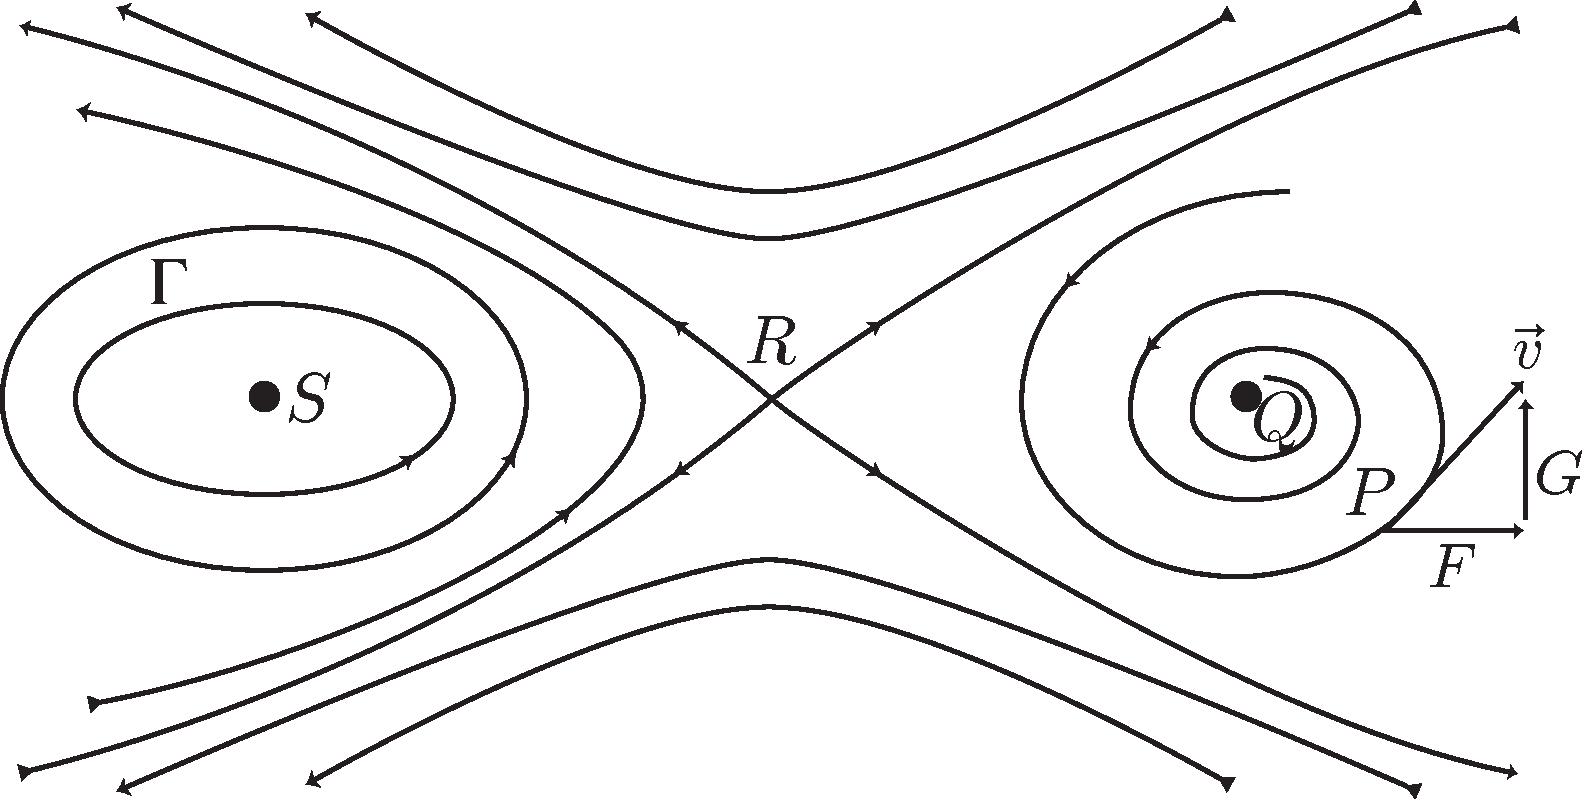
\includegraphics[width=4.5cm]{Graficos/figura1}
		\caption{ }
		\label{fig:M-1}
	\end{figure}

	
En la figura se pueden identificar lo siguiente:
	\begin{APAenumerate}
		\item Los puntos críticos,
		\item la disposición de las trayectorias cerca de los puntos críticos,
		\item la estabilidad o inestabilidad de los puntos críticos, es decir, si una partícula próxima a un punto crítico permanece cerca de él o se aleja hacia otra zona del plano,
		\item las trayectorias cerradas como la \(\Gamma\), corresponden a soluciones periódicas.
	\end{APAenumerate}

	\vspace{0.75\baselineskip}
	Como en general los sistemas no lineales no pueden resolverse explícitamente, el propósito de la teoría cualitativa siguiente es descubrir lo que sea posible acerca de los diagramas de fase a partir de las funciones \(F\) y \(G\).
\end{ejem}


%
%
%
\subsection{Tipos de puntos críticos y estabilidad}
%
%
%
Sea el sistema autónomo
\begin{equation}\label{m-4}
	\begin{cases}
		\dfrac{dx}{dt}=F(x,y) ,\vspace{0.3em}
		\\
		\dfrac{dy}{dt}=G(x,y),
	\end{cases}
\end{equation}
donde \(F=F(x,y)\) y \(G=G(x,y)\) son continuas, con derivadas parciales continuas en el plano de fase.

Sea \((x_0,y_0)\) un punto crítico aislado. Si \(\Gamma\big(x(t),y(t)\big)\) es una trayectoria del sistema, se dice que \(\Gamma\) tiende a \((x_0,y_0)\), cuando \(t\to\infty\) (o \(t\to-\infty\)), si:
\begin{equation}\label{m-5}
	\begin{cases}
		\lim_{t\to \infty} x(t) = x_0,
			 \\
		\lim_{t\to \infty} y(t) = y_0.
	\end{cases}
\end{equation}

\begin{observ}
	Si se cumple \eqref{m-5}, entonces \((x_0,y_0)\) es un punto crítico de \eqref{m-4}, además si \(\lim_{t\to\pm\infty}\dfrac{ y(t)-y_0}{x(t)-x_0}\), existe o es igual  a \(\pm\infty\), entonces se dice que \(\Gamma\) <<entra>> al punto crítico \((x_0,y_0)\) cuando \(t\to\infty\) o \(t\to-\infty\). Esto significa que la recta que une \((x_0,y_0)\) con \(P\) tiene una dirección determinada cuando \(t\to\infty\) o \(t\to-\infty\).
	
	Utilizando la regla de la cadena se tiene que \(\dfrac{dy}{dx}=\dfrac{G(x,y)}{F(x,y)}\) es la pendiente de la recta tangente de la trayectoria de \eqref{m-1} cuando \(F\) y \(G\) no se anulan simultáneamente; cuando se anulan simultáneamente, \((x_0,y_0)\) es un punto crítico y ninguna trayectoria pasa por él.
\end{observ}


\subsubsection{Tipos de puntos críticos}


Por facilidad y sin pérdida de generalidad se supondrá que \((0,0)\) es un punto crítico.

%
\vspace{0.75\baselineskip}
	\textbf{Nodos}\newline

\vspace{-1\baselineskip}
	\begin{figure}[H]
		\captionsetup{justification=centering, labelfont=footnotesize, font=footnotesize}
		\centering
		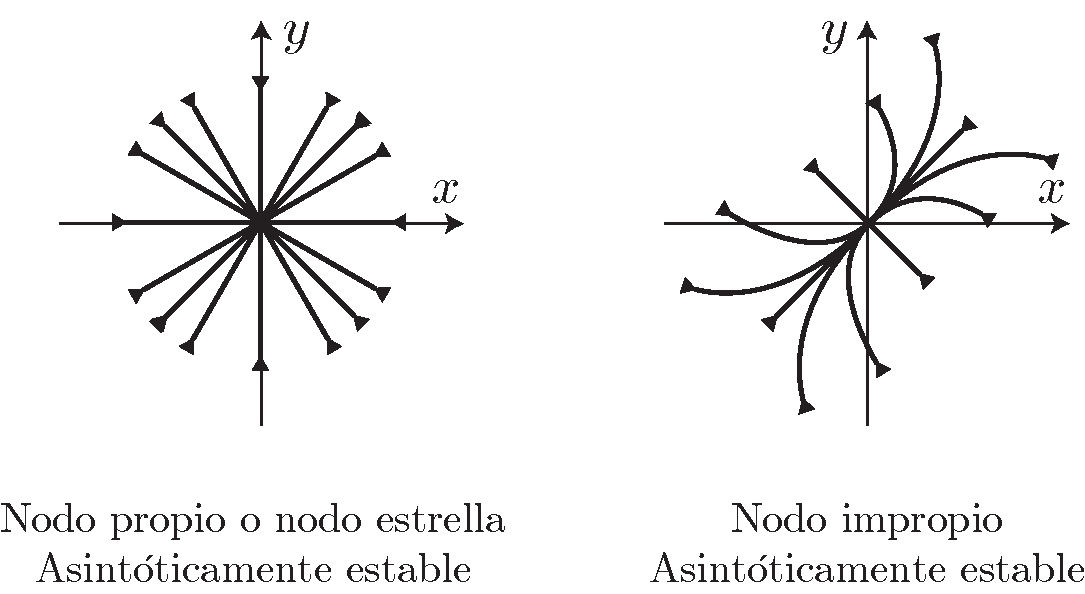
\includegraphics[scale=0.25]{Graficos/figura2}
		\caption{ }
		\label{fig:M-2}
	\end{figure}

Se distinguen dos tipos de nodos:
\begin{APAenumerate}
	\item \emph{\textbf{Nodos propios}}: en estos el retrato de fase está formado por semirectas donde todas entran (o todas salen) el punto crítico, se le llama también nodo estrella. Cuando tienden al punto cuando \(t\to\infty\), se dice que es un sumidero y cuando salen de él, o sea cuando tienden al punto cuando \(t\to-\infty\), se 	dice que es una fuente.
	
	\item \emph{\textbf{Nodo impropio}}: a un punto de este tipo tienden e incluso entran las trayectorias cuando \(t\to\infty\) (o \(t\to-\infty\)). Para este nodo existen cuatro trayectorias en forma de semirectas con extremos en el 	origen. Todas las demás trayectorias tienen el aspecto de ramas de parábola y al tender hacia el origen sus pendientes tienden a la pendiente de una de las semirectas.
\end{APAenumerate}

\vspace{-1\baselineskip}
	\begin{figure}[H]
		\captionsetup{justification=centering, labelfont=footnotesize, font=footnotesize}
		\centering
		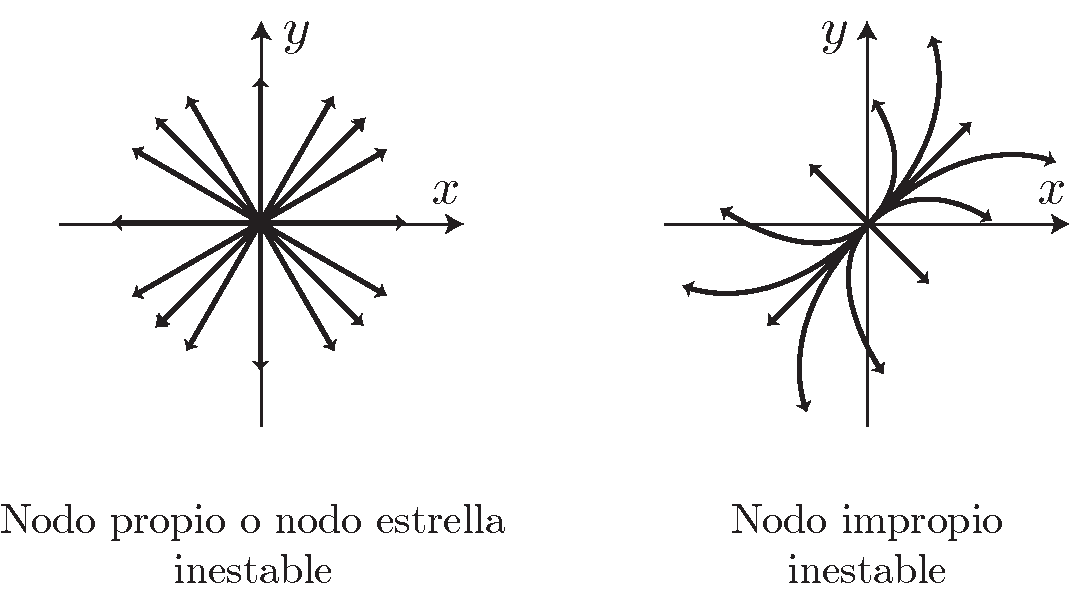
\includegraphics[scale=0.25]{Graficos/figura3}
		\caption{ }
		\label{fig:M-3}
	\end{figure}


\begin{ejem}
	Sea el sistema \(\nicefrac{dx}{dt}=x\), \(\nicefrac{dy}{dt}=-x+2y\) entonces \((0,0)\) es un punto crítico. La solución general es: 
	\[
		x(t)=c_1e^t	\yds	y(t)=c_1e^t+c_2e^{2t}.
	\]
	
	Cunado \(c_1=0 \Longrightarrow x=0\), \(y=c_2e^{2t}\) esto implica que la trayectoria es el eje \(Y\) positivo si \(c_2>0\) y el eje \(Y\) negativo si \(c_2>0\) y cada trayectoria tiende y  entra	 al origen cuando \(t\to-\infty\). Si \(c_2=0\) la trayectoria es la semirecta \(y=x\) con \(x<0\), \(c_1>0\), o también  la semirecta \(y=x\) con \(x<0\), \(c_1<0\). En estos casos ambas trayectorias tienden y entran al origen cuando \(t\to-\infty\).
	
	Si \(c_2=0\Longrightarrow x=c_1e^t\), \(y=c_1e^t\) y la trayectoria es la semirecta \(y=x\) con \(x>0\), \(c_1<0\) o también la
	semirecta \(y=x\) con \(x>0\), \(c_1>0\). En estos dos casos ambas trayectorias tienden y entran al origen cuando \(t\to-\infty\).
	
	Cuando \(c_1\neq0\), \(c_2\neq 0\), las trayectorias están sobre las parábolas \(y=x+\nicefrac{c_2}{c_1}x^2\) que entran al origen con	pendiente \(1\). Debe entenderse que estas trayectorias constan solo de una porción de la parábola, la parte con \(x>0\) si \(c_1>0\) y la parte \(x>0\) si \(c_1<0\).
	
	Nótese que \(\nicefrac{dy}{dx}=\nicefrac{(-x+2y)}{x}\): pendiente de la tangente a la trayectoria que pasa por \((x,y)\neq(0,0)\), resolviendo la EDO se encuentra \(y=x+cx^2\) que son las curvas (parábolas) sobre las que se apoyan las trayectorias, excepto las que están sobre el eje (ver figura \ref{fig:M-4}).
	
	\vspace{-1\baselineskip}
	\begin{figure}[H]
		\captionsetup{justification=centering, labelfont=footnotesize, font=footnotesize}
		\centering
		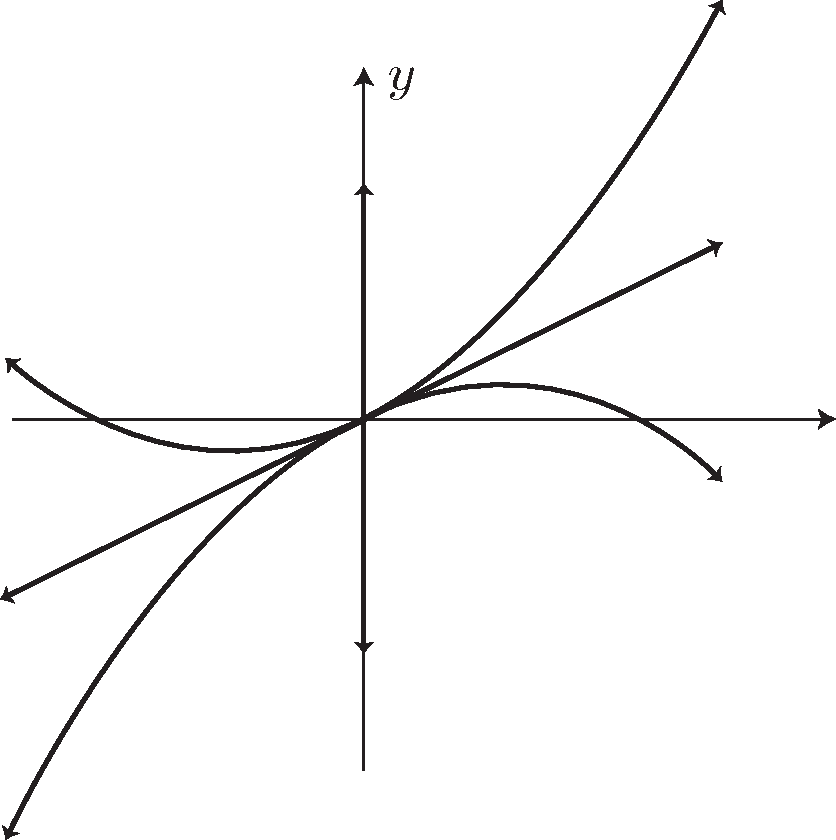
\includegraphics[width=4.5cm]{Graficos/figura4}
		\caption{Nodo impropio, inestable}
		\label{fig:M-4}
	\end{figure}
\end{ejem}



%
\vspace{0.75\baselineskip}
	\textbf{Punto de silla}\newline

\vspace{-1\baselineskip}
	\begin{figure}[H]
		\captionsetup{justification=centering, labelfont=footnotesize, font=footnotesize}
		\centering
		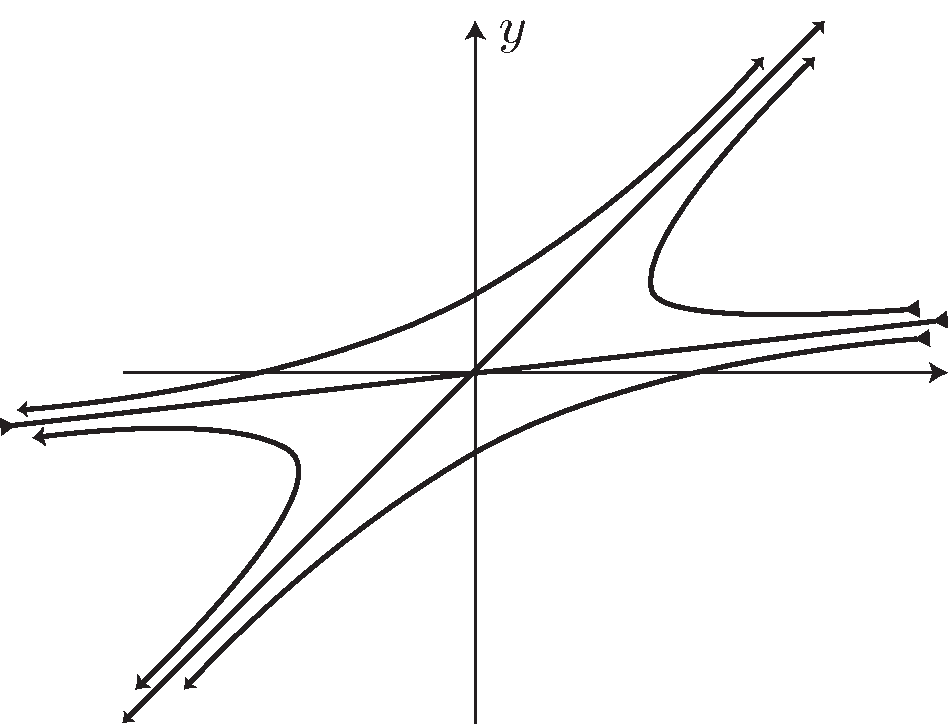
\includegraphics[width=4.5cm]{Graficos/figura5}
		\caption{Punto silla}
		\label{fig:M-5}
	\end{figure}

El origen es un punto silla si el retrato de fase muestra que a este punto tienden y hacia él entran dos semirectas con extremos en el origen cuando \(t\to\infty\) y hay otras dos semirectas que salen del origen cuando \(t\to-\infty\). Entre estas cuatro semirectas hay cuatro regiones, las cuales contienen una familia de trayectorias en forma de hipérbolas; estas trayectorias no tienden hacia el origen cuando , sino que son asintóticas a alguna de las semirectas. 

%
\vspace{0.75\baselineskip}
	\textbf{Centros (o vórtices)}\newline

\vspace{-1\baselineskip}
	\begin{figure}[H]
		\captionsetup{justification=centering, labelfont=footnotesize, font=footnotesize}
		\centering
		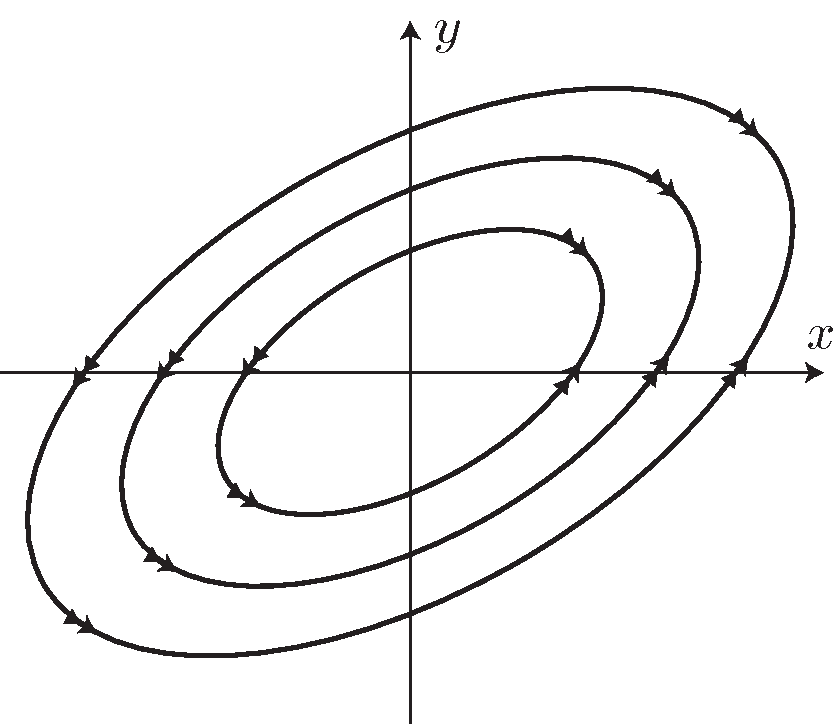
\includegraphics[width=4.5cm]{Graficos/figura6}
		\caption{Centro (estable)}
		\label{fig:M-6}
	\end{figure}

Es un punto crítico que está rodeado por una familia de trayectorias cerradas. Ninguna trayectoria tiende a él cuando \(t\to\pm\infty\).

\begin{ejem}
		Sea el sistema \(\nicefrac{dx}{dt}=-y\), \(\nicefrac{dy}{dt}=x\), el origen  es el único punto crítico.  Su solución general es:
		\[
		x(t) = -c_1 \sen t + c_2 \cos t 
		\yds
		y(t) = c_1 \sen t + c_2 \cos t.
		\]
		La solución que satisface las condiciones iniciales \(x(0)=1\), \(y(0)=0\) es  \(x=\cos t\), \(y=\sin t\), y la solución que satisface \(x(0)=0\), \(y(0)=1\) es \(x=-\sen t=\cos(t+\nicefrac{\pi}{2})\), \(y=\sen(t+\nicefrac{\pi}{2})\). Estas dos soluciones definen la misma trayectoria \(\Gamma\) que es la circunferencia \(x^2+y^2=1\) recorrida en sentido positivo (antihorario). En este caso \((0,0)\) es un centro.
		
		\vspace{-1\baselineskip}
	\begin{figure}[H]
		\captionsetup{justification=centering, labelfont=footnotesize, font=footnotesize}
		\centering
		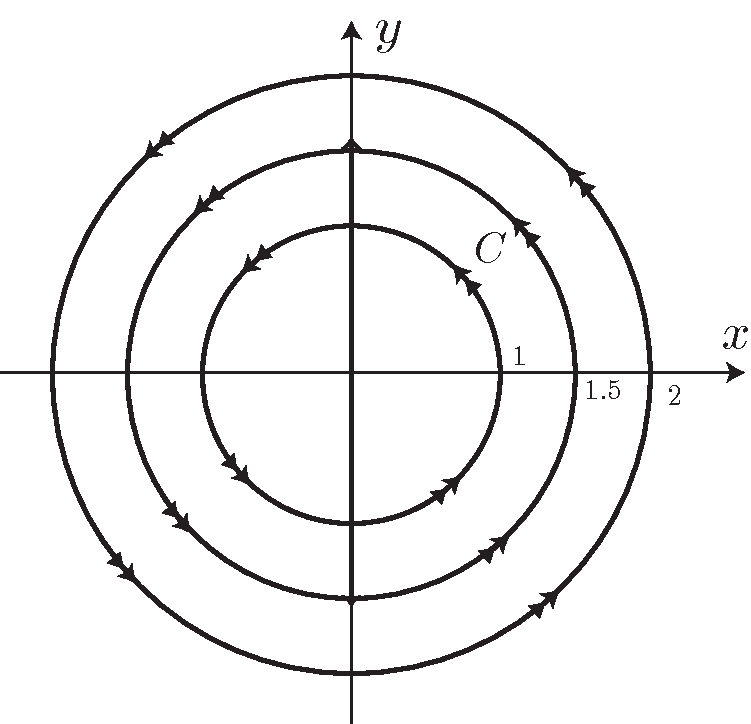
\includegraphics[width=4.5cm]{Graficos/figura7}
		\caption{Centro (estable)}
		\label{fig:M-7}
	\end{figure}		
	%
	\end{ejem}	

\newpage
%
%\vspace{0.75\baselineskip}
	\textbf{Focos}\newline

Un punto crítico se llama foco o punto espiral si el retrato de fase muestra que hacia él tienden (o salen de él) las trayectorias de una familia que gira en forma de espiral un número infinito de veces cuando \(t\to\pm\infty\).	Nótese que aunque las trayectorias tienden al origen, no entran a él en una dirección determinada, es decir, \(\displaystyle\lim_{t\to\infty}\nicefrac{dy}{dx}\) no existe.

\vspace{-1\baselineskip}
	\begin{figure}[H]
		\captionsetup{justification=centering, labelfont=footnotesize, font=footnotesize}
		\centering
		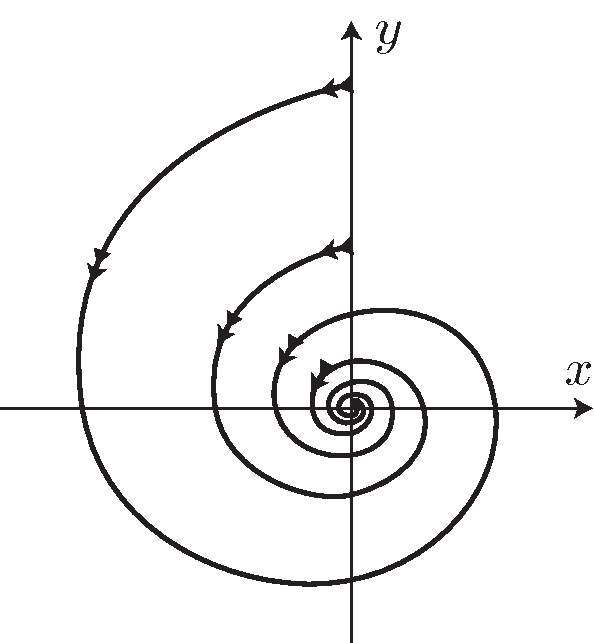
\includegraphics[width=4.5cm]{Graficos/figura8}
		\caption{Foco o espiral (asintóticamente estable)}
		\label{fig:M-8}
	\end{figure}

\begin{ejem}
	Sea \(a\) una constante arbitraria y considérese el sistema
	\[
	\begin{cases}
		\dfrac{dx}{dt}=ax - y,\vspace{0.3em}
		\\
		\dfrac{dy}{dt}=x+ay,
	\end{cases}
	\]

	Entonces \((0,0)\)es el único punto crítico, la ecuación diferencial de las trayectorias es:
			\[
			\dfrac{dx}{dy}=\dfrac{x+ay}{ax-y}.
			\]
			La cual en coordenadas polares queda: \(\nicefrac{dr}{d\theta}=ar\Longrightarrow r=ce^{a\theta}\) es la ecuación polar de las trayectorias.
			
			La dirección del recorrido se puede deducir del hecho que \(\nicefrac{dx}{dt}=-y\) cuando \(x=0\).
			
			Si \(a=0\)entonces el sistema se colapsa en \(\nicefrac{dx}{dt}=-y\), \(\nicefrac{dy}{dt}=x\) y se convierte en \(r=c\), que es la ecuación polar de la familia de circunferencias \(x^2+y^2=c^2\), en este caso se dice que cuando el parámetro \(a=0\)se ha producido una bifurcación, a este punto se lo llama de bifurcación, en esencia es un punto de donde las soluciones cambian cualitativamente de estable (o asintóticamente estables) a inestables o viceversa (ver figura \ref{fig:M-9}).
	
	\vspace{-1\baselineskip}
	\begin{figure}[H]
		\captionsetup{justification=centering, labelfont=footnotesize, font=footnotesize}
		\centering
		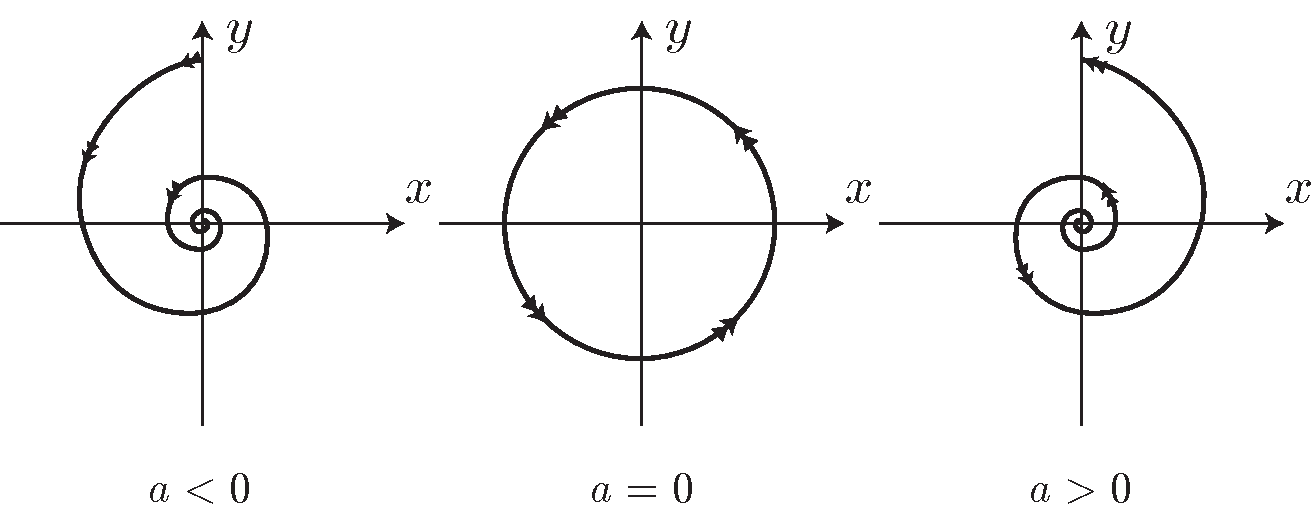
\includegraphics[scale=0.4]{Graficos/figura9}
	
		\footnotesize		
		\hspace{-2.5em}
		(a) Asin. estable	\qquad\qquad
		(b) Estable		\qquad\qquad
		(c) Inestable
		\caption{Bifurcación}
		\label{fig:M-9}
	\end{figure}
	
\end{ejem}


\subsubsection{Estabilidad}

\begin{definicion}
				Si \((0,0)\) es un punto crítico de \eqref{m-1}, se dice que es \emph{\textbf{estable}} si para cada \(R>0\) existe un \(r>0\), con \(r\leq R\), tal que toda trayectoria que está dentro del círculo \(x^2+y^2=r^2\), para algún  \(t=t_0\), permanece en el círculo \(x^2+y^2=R^2\) para todo \(t>t_0\), es decir, si todas las trayectorias que están suficientemente cerca al punto crítico permanecen cercanas a él (ver figura \ref{fig:M-10}).

\vspace{-1\baselineskip}
	\begin{figure}[H]
		\captionsetup{justification=centering, labelfont=footnotesize, font=footnotesize}
		\centering
		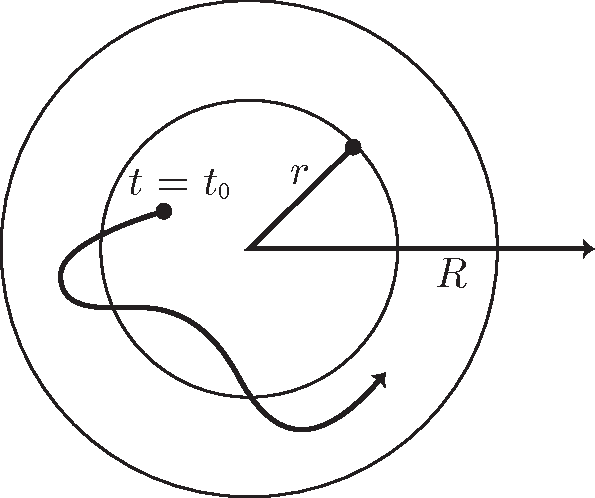
\includegraphics[width=4.5cm]{Graficos/figura10}
	
		\caption{}
		\label{fig:M-10}
	\end{figure}
\end{definicion}

\subsubsection{Asintóticamente estable}

\begin{definicion}
	Si el punto crítico es estable y existe un círculo \(x^2+y^2=r_0^2\), tal que toda trayectoria que está dentro de él para algún \(t=t_0\), tiende al origen cuando \(t\to\infty\).
\end{definicion}


\begin{definicion}
	Si el punto crítico no es estable, se dice que es inestable.
\end{definicion}






\newpage

%
%
%
\subsection{Puntos críticos y estabilidad para sistemas lineales}
%
%
%

Se considera el sistema
\begin{equation}\label{m-6}
	\begin{cases}
		\dfrac{dx}{dt}=a_1 x + b_1 y,\vspace{0.3em}
		\\
		\dfrac{dy}{dt}=a_2 x + b_2 y,
	\end{cases}
\end{equation}
el cual tiene  a \((0,0)\) como punto crítico. Se supondrá que:
\begin{equation}\label{m-7}
	\begin{vmatrix}
		a_1	&	b_1	\\
		a_2	&	b_2
	\end{vmatrix}
	=	a_1b_2-a_2b_1\neq 0.
\end{equation}
Por tanto \((0,0)\) es el único punto crítico.

El sistema tiene una solución no trivial de la forma:
\vspace{0.5\baselineskip}
\begin{APAenumerate}
	\item \( \begin{aligned}[t]
	X_1 = \binom{x}{y}
		= e^{m_1 t } \binom{A_1}{B_1}
	;
	\qquad
	X_2 = \binom{x}{y}
		= e^{m_2 t } \binom{A_2}{B_2},
	\end{aligned}
	\)
	donde \(m_{1,2}\) son raíces distintas de la ecuación cuadrática: 
	\begin{equation}\label{m-8}
		m^2-(a_1+b_1)m+(a_1b_2-a_2b_1)=0.
	\end{equation}
	Que se conoce como ecuación característica del sistema, y \(\binom{A_1}{B_1}\), \(\binom{A_2}{B_2}\) son los vectores propios asociados a los valores propios \(m_{1,2}\). La condición \eqref{m-7} implica que \(m\neq 0\).
	
	\vspace{1\baselineskip}
	\item O de la forma:
	\( \begin{aligned}[t]
	X_1 = \binom{x}{y}
		= e^{m t } \binom{A}{B}
	;
	\qquad
	X_2 = \binom{x}{y}
		= e^{m t } \left[ \binom{A_1}{B_1} + t \binom{A}{B} \right]
	\end{aligned},
	\)
	donde \(\binom{A}{B}\) es el vector propio asociado al valor propio \(m\) de multiplicidad 2, y  \(\binom{A_1}{B_1}\) es el vector propio generalizado de rango 2 de \(m\).
\end{APAenumerate}

%
\subsubsection{Caracterización de la naturaleza del punto crítico}

\begin{teorema}\label{teo-1}
	Sean \(m_1\) y \(m_2\) las raíces del polinomio característico. La naturaleza del punto crítico esta determinada por estas raíces.
\end{teorema}

Casos principales:
\begin{itemize}[leftmargin=15pt]
	\item[A:] Si las raíces \(m_1\) y \(m_2\) son reales, distintas y del mismo signo, entonces es un nodo.
	\item[B:] Si las raíces \(m_1\) y \(m_2\) son reales, distintas y de signos opuestos, entonces es un punto de silla.
	\item[C:] Si las raíces \(m_1\) y \(m_2\) son complejas conjugadas pero no imaginarias puras, entonces es un foco.
	\item[D:] Si las raíces \(m_1\) y \(m_2\) son reales e iguales, entonces es un nodo.
	\item[E:] Si las raíces \(m_1\) y \(m_2\) son imaginarias puras, entonces es un centro.
\end{itemize}

\newpage

\begin{observ}
	Para el Caso A, se puede tener:
	
	Si \(m_1<m_2<0\) se tiene un nodo impropio (asintóticamente estable)
	\vspace{-1\baselineskip}
	\begin{figure}[H]
		\captionsetup{justification=centering, labelfont=footnotesize, font=footnotesize}
		\centering
		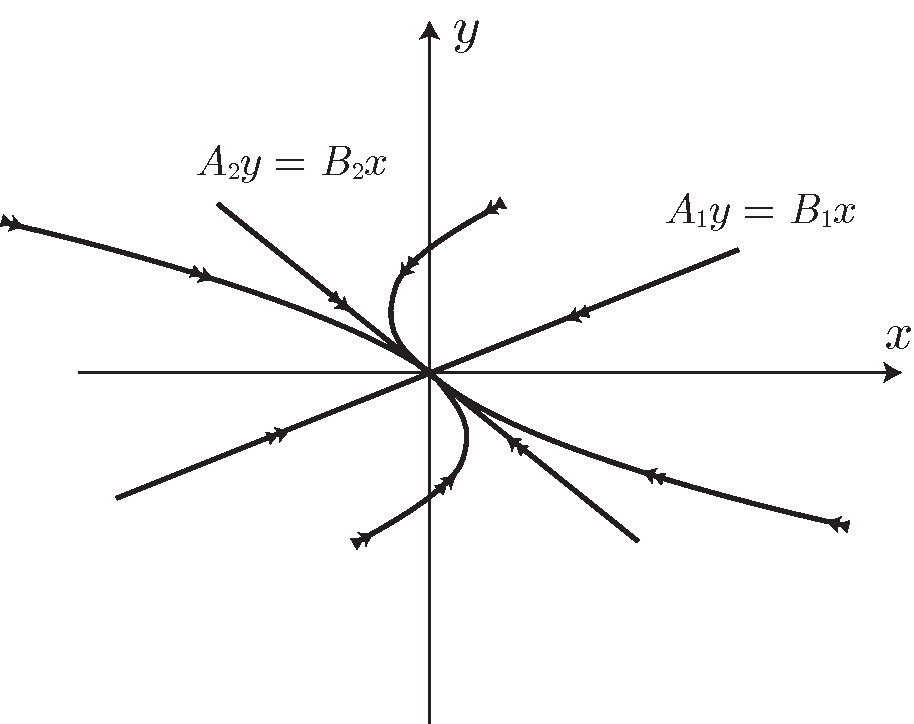
\includegraphics[width=4.5cm]{Graficos/figura11}
	
		\caption{Nodo impropio (asintóticamente estable)}
		\label{fig:M-11}
	\end{figure}
	
	Si \(m_1>m_2>0\) se tiene un nodo impropio (asintóticamente inestable)
	\vspace{-1\baselineskip}
	\begin{figure}[H]
		\captionsetup{justification=centering, labelfont=footnotesize, font=footnotesize}
		\centering
		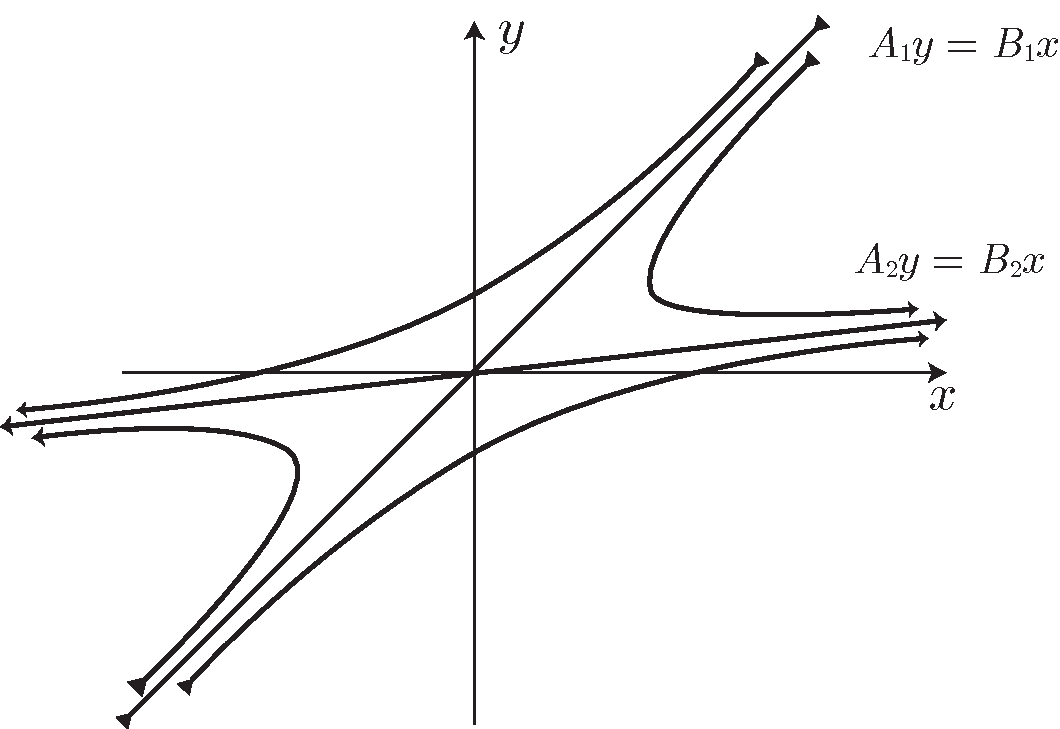
\includegraphics[width=4.5cm]{Graficos/figura12}
	
		\caption{Punto silla (inestable)}
		\label{fig:M-12}
	\end{figure}
	
	Para el Caso B, se tiene un punto de silla
	\vspace{-1\baselineskip}
	\begin{figure}[H]
		\captionsetup{justification=centering, labelfont=footnotesize, font=footnotesize}
		\centering
		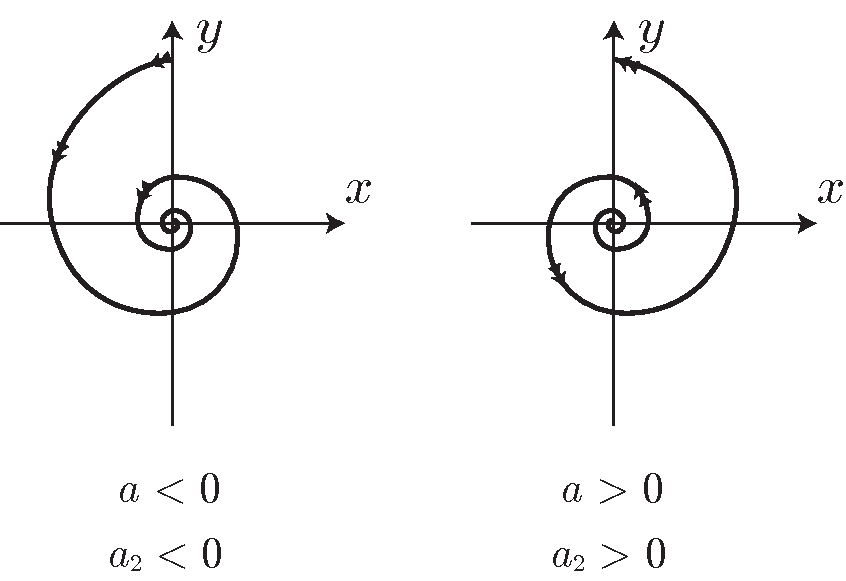
\includegraphics[width=4.5cm]{Graficos/figura13}
	
		\caption{Focos (asintóticamente estables)}
		\label{fig:M-13}
	\end{figure}
	
	Para el Caso D, se tiene  dos casos:
	\begin{APAenumerate}
		\item \(a_1=b_2\neq 0\), \(a_2=b_1=0\) se tiene un nodo propio o nodo estrella asintóticamente estable
		\vspace{-1\baselineskip}
	\begin{figure}[H]
		\captionsetup{justification=centering, labelfont=footnotesize, font=footnotesize}
		\centering
		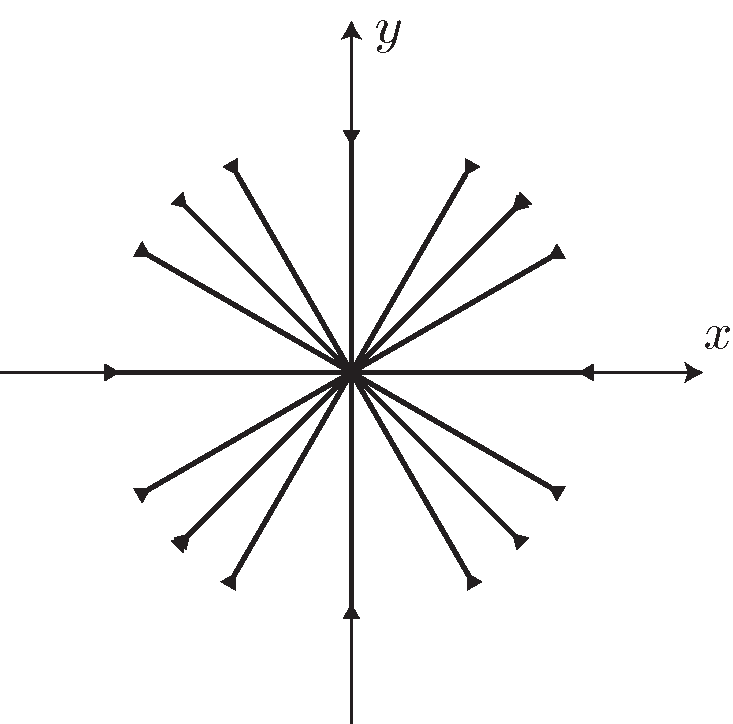
\includegraphics[width=4.5cm]{Graficos/figura14}
	
		\caption{Nodo propio o nodo estrella (asintóticamente estable)}
		\label{fig:M-14}
	\end{figure}
		
		
		\item Todas las demás posibilidades dan como resultado un nodo impropio asintóticamente estable
		\vspace{-1\baselineskip}
	\begin{figure}[H]
		\captionsetup{justification=centering, labelfont=footnotesize, font=footnotesize}
		\centering
		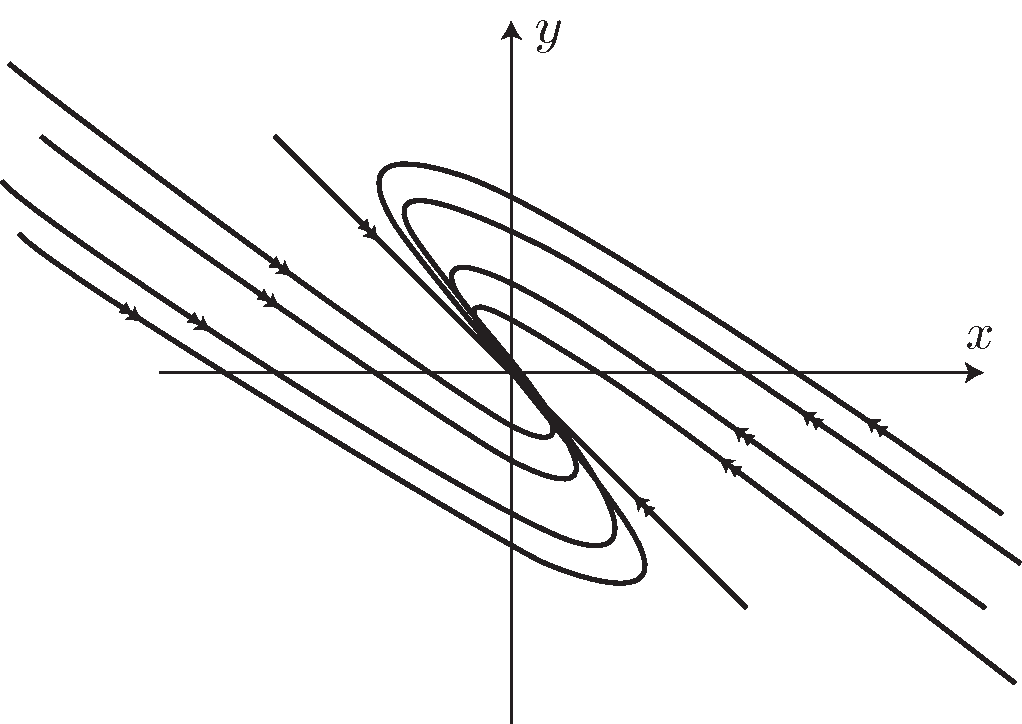
\includegraphics[width=4.5cm]{Graficos/figura15}
	
		\caption{Nodo impropio (asintóticamente estable)}
		\label{fig:M-15}
	\end{figure}
	\end{APAenumerate}

Para el Caso E, el punto \((0,0)\) es un centro estable
\vspace{-1\baselineskip}
	\begin{figure}[H]
		\captionsetup{justification=centering, labelfont=footnotesize, font=footnotesize}
		\centering
		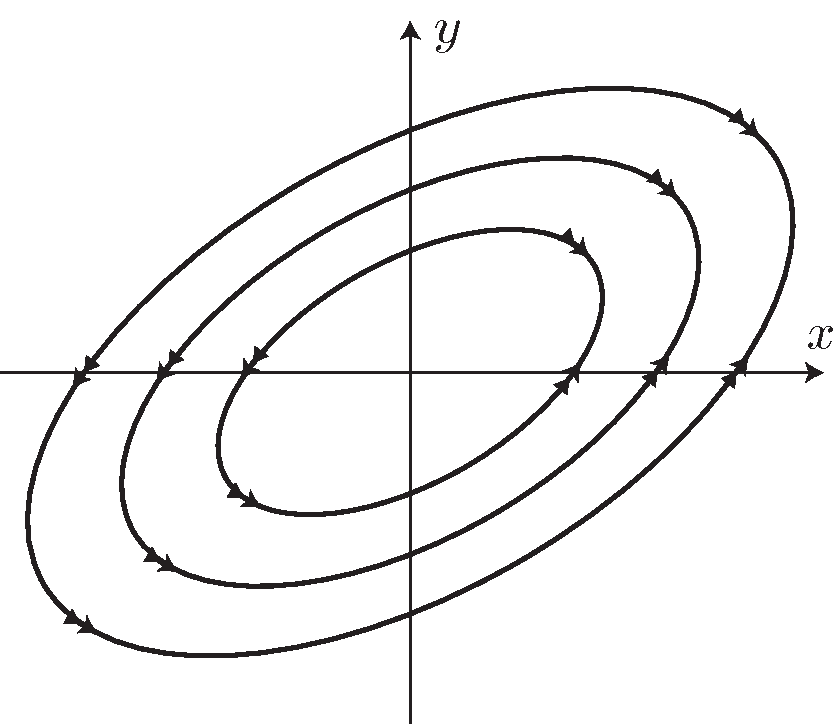
\includegraphics[width=4.5cm]{Graficos/figura6}
	
		\caption{Centro (estable)}
		\label{fig:M-16}
	\end{figure}
\end{observ}


%
\subsubsection{Criterio de estabilidad}


\begin{teorema}\label{teo-2}
	El punto crítico \((0,0)\) del sistema es estable si y solo si  ambas raíces de la ecuación auxiliar: \(m^2-(a_1+b_2)m+(a_1b_2-a_2b_a)=0\) tienen partes reales no positivas, y es  asintóticamente estable si y solo si 	ambas raíces tienen partes reales negativas.
\end{teorema}

En efecto: si la ecuación auxiliar se escribe de la forma:
\[
(m-m_1)(m-m_2)=m^2-(m_1+m_2)m+m_1m_2=m^2+pm+1=0,
\]
entonces los cinco casos anteriores se pueden escribir en términos de \(p\) y \(q\) y para ello se utiliza el plano \(pq\).

El eje \(p\) está excluido ya que \(q=m_1m_2=a_1b_2-a_2b_1\neq 0\). Por tanto toda la información se puede extraer de \(m_{1,2}=\nicefrac{\big(-p\pm\sqrt{p^2-4q}\big)}{2}\).
\vspace{-1\baselineskip}
	\begin{figure}[H]
		\captionsetup{justification=centering, labelfont=footnotesize, font=footnotesize}
		\centering
		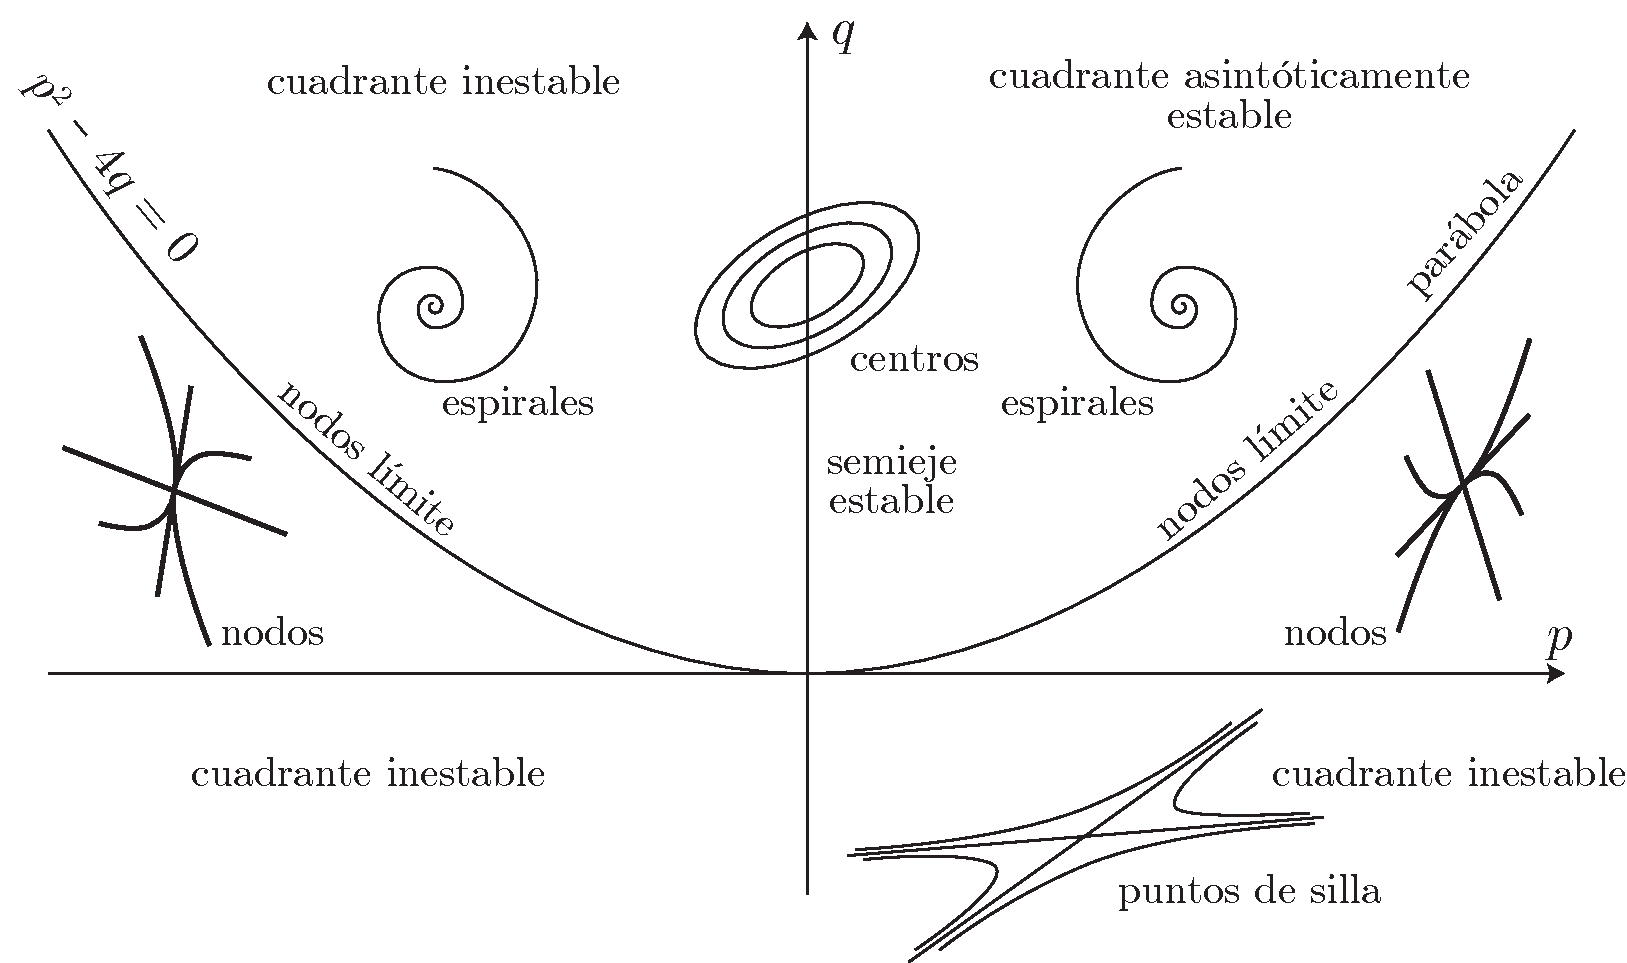
\includegraphics[scale=0.35]{Graficos/figura17}
	
		\caption{ }
		\label{fig:M-17}
	\end{figure}

De la figura \ref{fig:M-17} se tiene que:
\begin{APAitemize}
	\item Por encima de la parábola \(p^2-4q=0\) se tiene que \(p^2-4q<0\). Luego \(m_{1,2}\) son números 	complejos y estos son imaginarios puros si y solo si \(p=0\); estos son los caso C y E de focos y centros.
	\item Por debajo del eje \(p\) se tiene \(q<0\) lo que implica que las raíces son reales distintas y de signos opuestos, por tanto es un punto silla o sea el caso B.
	\item La zona entre la parábola y el eje \(p\) (excluido este eje e incluyendo a la parábola), se caracteriza porque \(p^2-4q\geq 0\), \(q>0\),  de donde las raíces son reales y del mismo signo y sobre la parábola	son iguales, por tanto son nodos y son los casos A y D.
	\item El primer cuadrante excluyendo a los ejes, es una región con estabilidad asintótica; el eje positivo \(q\) corresponde a centros y por tanto es estable; el segundo, tercero y cuarto cuadrante son regiones inestables.
\end{APAitemize}


%
\subsubsection{Criterio de estabilidad asintótica}

\begin{teorema}
	El punto critico \((0,0)\) es asintóticamente estable si y solo si  los coeficientes \(p=-(a_1+b_2)\), \(q=a_1b_2-a_2b_1\) de la ecuación auxiliar son ambos positivos.
\end{teorema}

%\newpage

%
%
%
\subsection{Criterio de estabilidad por el método de Liapunov}
%
%
%
Considerando el sistema autónomo
\begin{equation}\label{m-9}
	\begin{cases}
		\dfrac{dx}{dt}=F(x,y) ,\vspace{0.3em}
		\\
		\dfrac{dy}{dt}=G(x,y),
	\end{cases}
\end{equation}

Suponiendo que tiene un punto crítico aislado; sea \((0,0)\) dicho punto (un punto crítico \(( x_0 , y_0 )\) se puede
llevar al origen por medio de una traslación). Sea \(\Gamma\big(x(t),y(t)\big)\) una trayectoria del sistema y sea \(E( x , y )\) una función continua con primeras derivadas parciales continuas en una región que contiene a la trayectoria. Si un punto \(( x, y )\) se mueve a lo largo de la trayectoria de acuerdo a las ecuaciones: \(x = x ( t )\), \(y = y ( t )\), entonces: 
\[
	E(x,y)=E\big(x(t),y(t)\big)=E(t).
\]
Es una función de \(t\) sobre \(\Gamma\), su razón de cambio es:
\begin{equation}\label{m-10}
	E'(x,y)=\dfrac{dE}{dt}=\dfrac{\partial E}{\partial x}\dfrac{dx}{dt}+\dfrac{\partial E}{\partial y}\dfrac{dy}{dt}=\dfrac{\partial E}{dx}F+\dfrac{\partial E}{\partial y}G.
\end{equation}
Esta fórmula es la idea principal de Liapunov.

\begin{definicion}
	Suponiendo que E \(( x , y )\) es continua y tiene primeras derivadas parciales continuas en una región que contiene al origen. Si \(E ( 0 , 0 ) = 0\) y
	\begin{APAenumerate}
		\item si \(E(x,y)>0\) y \((x,y)\neq(0,0)\), se dice que \(E(x,y)\) es definida positiva,
		\item si \(E(x,y)<0\) y \((x,y)\neq(0,0)\), se dice que \(E(x,y)\) es definida negativa,
		\item si \(E(x,y)\geq 0\) y \((x,y)\neq(0,0)\), se dice que \(E(x,y)\) es semidefinida positiva,
		\item si \(E(x,y)\leq 0\) y \((x,y)\neq(0,0)\), se dice que \(E(x,y)\) es semidefinida negativa.
	\end{APAenumerate}
\end{definicion}

\begin{observ}\quad
	\begin{APAitemize}
		\item \(E(x,y)=ax^{2m} + by^{2n}\) con \(a>0\), \(b>0\) y \(m\), \(n\) enteros positivos, es definida positiva.
		\item \(E(x,y)\) es definida negativa si y solo si \(-E(x,y)\) es definida positiva.
		\item Si \(E(x,y)\) es definida positiva, entonces \(z=E(x,y)\) es la ecuación de una superficie que podría parecerse a un paraboloide abierto hacia arriba y tangente al plano \(xy\) en el origen (ver figura \ref{fig:M-18}).
		%
		\vspace{-1\baselineskip}
	\begin{figure}[H]
		\captionsetup{justification=centering, labelfont=footnotesize, font=footnotesize}
		\centering
		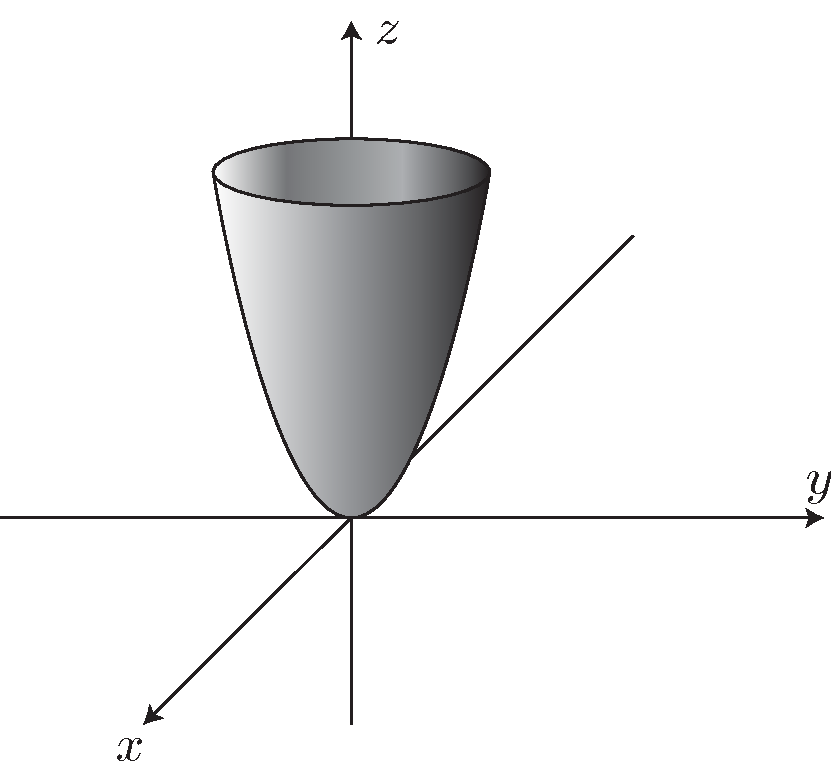
\includegraphics[scale=0.35]{Graficos/figura18}
	
		\caption{ }
		\label{fig:M-18}
	\end{figure}	\end{APAitemize}
\end{observ}


\subsubsection{Función de Liapunov}

\begin{definicion}
	Se dice que \(E(x,y)\) es una \emph{\textbf{función de Liapunov}} para el sistema autónomo, si:
	\begin{APAitemize}
		\item \(E(x,y)\) es continua, con primeras derivadas parciales continuas en una región que contiene al 	origen
		\item \(E(x,y)\) es definida positiva
		\item Existe la derivada de \(E\) a lo largo de trayectorias u órbitas del sistema y sea menor o igual que cero sobre la trayectoria, es decir, existe la derivada:
		\[
		\dfrac{\partial E}{\partial x}F+\dfrac{\partial E}{\partial y}G=E'\leq 0.
		\]
		\item Cuando \(\nicefrac{\partial E}{\partial x}F+\nicefrac{\partial E}{\partial y}G=E'<0\) se dice que \(E(x,y)\), se dice que es una \emph{\textbf{función de Liapunov}}	estricta.
	\end{APAitemize}
\end{definicion}


\subsubsection{Criterio de Liapunov}

\begin{teorema}\quad
	\begin{APAenumerate}
		\item Si existe una función de Liapunov para el sistema, entonces el punto crítico \(( 0 , 0 )\) es estable.
		\item Si existe una función de Liapunov estricta para el sistema, entonces \((0,0)\) es un punto crítico asintóticamente estable.
		\item Si \(E'(x,y)\) es definida positiva, entonces el punto crítico \((0,0)\) es inestable.
	\end{APAenumerate}
\end{teorema}

\begin{ejem}
	La ecuación diferencial de una masa \(m\) sujeta a un resorte de constante \(k\) , en un medio que ofrece un amortiguamiento de coeficiente \(C\) es:
	\[
	m\dfrac{d^2x}{dt^2}+C\dfrac{dx}{dt}+kx=0.
	\]
	Analizar la estabilidad de su punto crítico.
\end{ejem}
\begin{proof}[Solución]
		El sistema autónomo equivalente es:
		\[
		\begin{cases}
		\dfrac{dx}{dt}=y,\vspace{0.3em}
		\\
		\dfrac{dy}{dt}=-\dfrac{k}{m}x-\dfrac{C}{m}y.
	\end{cases}
		\]
		Su único punto crítico es \((0,0)\). La energía cinética es \(\nicefrac{1}{2}my^2\) y la energía potencial (o energía almacenada en el muelle) es \(\int_{0}^{x}kx\,dx=\nicefrac{1}{2}kx^2\), luego la energía total es: \(E(x,y)=\nicefrac{1}{2}my^2+\nicefrac{1}{2}kx^2\), la cual es definida positiva.
		
		Como \(\nicefrac{\partial E}{\partial x}F+\nicefrac{\partial E}{\partial y}G=kxy+my\left(-\nicefrac{k}{m}x-\nicefrac{C}{m}y\right)=-Cy^2\leq 0\). Se tiene que \(E(x,y)\) es una función de Liapunov para el sistema y por tanto \((0,0)\) es estable.
		
		Se sabe que si \(C>0\) el punto crítico \((0,0)\) es asintóticamente estable, pero la función de Liapunov no detecta este hecho.
\end{proof}

\begin{ejem}[Resorte no lineal]
	Este es un ejemplo de masa \(m=1\) sujeta a un resorte no lineal, en el cual la fuerza restauradora es una función de la distancia de la masa al origen, sea \(-f(x)\) una función no lineal que representa la fuerza restauradora tal que \(f(0)=0\) y \(xf(x)>0\), \(x\neq 0\); no hay fricción. La ecuación de su movimiento es: \(\nicefrac{d^2x}{dt^2}+f(x)=0\). Analizar la estabilidad de su punto crítico.
\end{ejem}
\begin{proof}[Solución]
		El sistema autónomo equivalente es: 
		\[
			x'=y \yds y'=-f(x).
		\]
		
		Su único punto crítico es \((0,0)\). La energía cinética es \(\nicefrac{1}{2}x'^2=\nicefrac{1}{2}y^2\) y la energía potencial es: 
		\[
		F(x)=\displaystyle\int_{0}^{x}f(x)\,dx.
		\]
		Y la energía total es:
		\[
		E(x,y)=F(x)+\dfrac{1}{2}y^2.
		\]
		Como \(x\) y \(f(x)\) tienen el mismo signo entonces \(F(x)\geq0\) y por tanto \(E(x,y)\) es definida positiva. Además,
		\[
		E'(x,y)=F'(x)x'+yy'=f(x)y+y\big(-f(x)\big)=0.
		\]
		Es decir, es semidefinida negativa y por el teorema el punto crítico \((0,0)\) es estable. Igual que sucede con un resorte lineal, se puede demostrar que este punto crítico es un centro.
\end{proof}


\begin{ejem}
	Analizar la estabilidad del sistema:
	\[
	\begin{cases}
		x'=-x-\dfrac{x^3}{3}-x\sen y,
		\\
		y'=-y-\dfrac{y^3}{3}.
	\end{cases}
	\]
\end{ejem}
	\begin{proof}[Solución]
		El origen \((0,0)\) es el único punto crítico. Sea \(E(x,y)=\nicefrac{1}{2}(x^2+y^2)\), luego
		\begin{align*}
			E'(x,y)&=x\left(-x-\dfrac{x^3}{3}-x\sen y\right)+y\left(-y-\dfrac{y^3}{3}\right)\\
				&=-x^2-\dfrac{x^4}{3}-y^2-\dfrac{y^4}{3}-x^2\sen y\\
				&\leq -\dfrac{x^4}{3}-y^2-\dfrac{y^4}{3}<0.
		\end{align*}
		Es decir, \(E'\) es definida negativa, por tanto \((0,0)\) es asintóticamente estable.
	\end{proof}


\begin{ejem}
	Analizar la estabilidad del punto crítico del sistema:
	\[
	\begin{cases}
		x'=-2xy
		\\
		y'=x^2-y^2
	\end{cases}
	\]
\end{ejem}
	\begin{proof}[Solución]
		El origen \((0,0)\) es un punto crítico asilado. Sea \(E(x,y)=ax^{2m}+by^{2m}\), luego:
		\begin{align*}
			E'(x,y)&=2amx^{2m-1}(-2xy)+2by^{2n-1}(x^2-y^2)\\
				&=\left(-4amx^{2n}y+2bnx^2y^{2n-1}\right)-2nby^{2n+2} .
		\end{align*}
		Si: \(m=1\), \(n=1\), \(a=1\), \(b=2\) el paréntesis se anula, y se tiene: \(E(x,y)=x^2+2y^2\) es definida positiva y \(\nicefrac{\partial E}{\partial x}F+\nicefrac{\partial E}{\partial y}G=-4y^2\) es semidefinida negativa, de donde: \((0,0)\) es estable.
	\end{proof}



\begin{teorema}
	La función \(f(x,y)=ax^2+bxy+cy^2\) es:
	\begin{APAitemize}
		\item definida positiva si y solo si  \(a>0\) y \(b^2-4ac<0\),
		\item semidefinida positiva si y solo si \(a>0\) y \(b^2-4ac\leq 0\),
		\item definida negativa si y solo si \(a<0\) y \(b^2-4ac<0\),
		\item semidefinida negativa si y solo si \(a<0\) y \(b^2-4ac\leq 0\).
	\end{APAitemize}
\end{teorema}

%\newpage

%
%
%
\subsection{Linealización de sistemas no lineales}
%
%
%
Considere el sistema autónomo
\begin{equation}\label{m-11}
	\begin{cases}
		x'=F(x,y) ,
		\\
		y'=G(x,y),
	\end{cases}
\end{equation}
con un punto crítico asilado en \((x_0,y_0)\) (es decir \(F(x_0,y_0)=G(x_0,y_0)=0\)). Si \(F(x,y)\) y \(G(X,y)\) se pueden desarrollar en series de potencias alrededor de \((x_0,y_0)\), entonces si: \(u=x-x_0\), \(v=y-y_0\), entonces:
\begin{align}
	u'=x'&=F(x_0+u,y_0+v)\nonumber\\
		&=F(x_0,y_0)+u\dfrac{\partial F}{\partial x}(x_0,y_0)+v\dfrac{\partial F}{\partial y}(x_0,y_0)+\mathcal{O}(u,v,uv)\nonumber\\
		&=u\dfrac{\partial F}{\partial x}+v\dfrac{\partial F}{\partial y}+\mathcal{O}(u,v,uv)\label{m-12}
\end{align}
Similar:
\begin{equation}\label{m-13}
	v'=y'=u\dfrac{\partial G}{\partial x}+v\dfrac{\partial G}{\partial y}+\mathcal{O}'(u,v,uv).
\end{equation}
En forma matricial, se tiene que:
\begin{equation}\label{m-14}
	\begin{pmatrix} u' \\ v' \end{pmatrix}
	= \begin{pmatrix} \dfrac{\partial F}{\partial x} & \dfrac{\partial F}{\partial y} \\
\dfrac{\partial G}{\partial x} & \dfrac{\partial G}{\partial y} \end{pmatrix} \begin{pmatrix} u \\ v\end{pmatrix}+\begin{pmatrix} \mathcal{O}(u,v,uv) \\ \mathcal{O}'(u,v,uv)\end{pmatrix}.
\end{equation}

La matriz
\[
	J(F,G)(x_0,y_0)=\begin{pmatrix} \dfrac{\partial F}{\partial x}(x_0,y_0) & \dfrac{\partial F}{\partial y}(x_0,y_0) \\[1em]
\dfrac{\partial G}{\partial x}(x_0,y_0) & \dfrac{\partial G}{\partial y}(x_0,y_0)\end{pmatrix}
\]
se llama la \emph{\textbf{matriz Jacobiana}} del sistema evaluada en el punto crítico \((x_0,y_0)\). Cuando \(|u|\), \(|v|\) son pequeños, es decir, cuando \((u,v)\to(0,0)\) los términos de segundo orden y de orden superior son pequeños. Despreciando estos términos, se conjetura que el comportamiento cualitativo de \eqref{m-14} es similar al del sistema lineal asociado:
\begin{equation}\label{m-15}
	\begin{pmatrix} u' \\ v' \end{pmatrix}=\begin{pmatrix} \dfrac{\partial F}{\partial x} & \dfrac{\partial F}{\partial y} \\ \dfrac{\partial G}{\partial x} & \dfrac{\partial G}{\partial y} \end{pmatrix}	\begin{pmatrix} u \\ v \end{pmatrix},
\end{equation}
donde:
\[
\det\begin{pmatrix} \dfrac{\partial F}{\partial x}(x_0,y_0) & \dfrac{\partial F}{\partial y}(x_0,y_0) \\[1em]
\dfrac{\partial G}{\partial x}(x_0,y_0) & \dfrac{\partial G}{\partial y}(x_0,y_0)\end{pmatrix}\neq 0.
\]
Nótese que si \((x_0,y_0)\) es un punto crítico del sistema  de coordenadas \(XY\) entonces \((0,0)\) es el punto crítico en el nuevo sistema de coordenadas \(UV\). El proceso anterior de sustituir el sistema original por el  sistema lineal, se llama \emph{\textbf{linealización}} en el punto \((x_0,y_0)\).

Si se denota \(a_1=\nicefrac{\partial F}{\partial x}(x_0,y_0)\), \(b_1=\nicefrac{\partial F}{\partial y}(x_0,y_0)\), \(a_2=\nicefrac{\partial G}{\partial x}(x_0,y_0)\), \(b_2=\nicefrac{\partial G}{\partial y}(x_0,y_0)\), \(F(x_0,y_0)=0\) y \(G(x_0,y_0)=0\). El sistema puede ponerse de la forma:
\begin{equation}\label{m-16}
	\begin{cases}
		\dfrac{dx}{dt}= a_1x+b_1 y+f(x,y),	\vspace{0.3em}
		\\[1em]
		\dfrac{dy}{dt}= a_2 x+b_2 y+g(x,y).
	\end{cases}
\end{equation}
Suponiendo que
\begin{equation}\label{m-17}
	\det\begin{pmatrix} a_1 & b_1 \\ a_2 & b_2 \end{pmatrix} \neq 0,
\end{equation}
de tal manera que el sistema lineal asociado tiene a \((0,0)\) como punto crítico asilado y suponiendo que \(f\) y \(g\) son funciones continuas con primeras derivadas parciales continuas para todo \((x,y)\) y que
\begin{align}\label{m-18}
	\lim_{(x,y)\to(0,0)}\dfrac{f(x,y)}{\sqrt{x^2+y^2}} &= 0,
	\\
	\lim_{(x,y)\to(0,0)}\dfrac{g(x,y)}{\sqrt{x^2+y^2}}&= 0.
\end{align}
Estas dos últimas condiciones implican (por la continuidad) que \(f(0,0)=0\) y \(g(0,0)=0\), es decir, \((0,0)\) es un punto crítico. Se puede demostrar que es aislado. Con las restricciones indicadas se le llama \emph{\textbf{punto crítico simple}} de \eqref{m-16}.

Cuando se cumplen las condiciones \eqref{m-17} y \eqref{m-18}, se dice que  el sistema \eqref{m-16} es casi lineal o cuasi-lineal.

\begin{ejem}
	Comprobar que se cumplen las condiciones anteriores para el sistema:
	\[
	\begin{cases}
		\dfrac{dx}{dt}= -2x+3y+xy,	\vspace{0.3em}
		\\
		\dfrac{dy}{dt}= -x+y-2xy^2.
	\end{cases}
	\]
\end{ejem}
\begin{proof}[Solución]
		\[
		\det\begin{pmatrix} a_1 & b_1 \\ a_2 & b_2 \end{pmatrix}=\det\begin{pmatrix} -2 & 3 \\ -1 & 1 \end{pmatrix}=1\neq 0.
		\]
		Al usar coordenadas polares:
		\[
			\dfrac{|f(x,y)|}{\sqrt{x^2+y^2}}=\dfrac{|r^2\sin\theta\cos\theta|}{r}\leq r
			\yds
			\dfrac{|g(x,y)|}{\sqrt{x^2+y^2}}=\dfrac{|2r^3\sin^2\theta\cos\theta|}{r}\leq 2r^2.
		\]
		Cuando \((x,y)\to (0,0)\) se tiene:
		\[
			\lim_{r\to 0}\dfrac{f(x,y)}{r} = 0 \yds
			\lim_{r\to 0}\dfrac{g(x,y)}{r}=0.
		\]
		Luego \((0,0)\) es un punto crítico simple del sistema.
\end{proof}

\newpage

\subsubsection{Tipos de punto crítico para sistemas no lineales}

\begin{teorema}\label{teo-6}
	Sea \((0,0)\) un punto crítico simple del sistema no lineal \eqref{m-16} y considere el sistema lineal asociado:
	\[
		\begin{cases}
			\dfrac{dx}{dt}=a_1 x + b_1 y,	\vspace{0.3em}
			\\
			\dfrac{dy}{dt}= a_2 x + b_2 y.
		\end{cases}
	\]
	Si el punto crítico \((0,0)\) del sistema asociado pertenece a alguno de los tres casos principales del  teorema \eqref{teo-1}, entonces el punto crítico \((0,0)\) es del mismo tipo para el sistema no lineal.
\end{teorema}

\begin{ejem}
	En el ejemplo anterior, analizar el punto crítico.
\end{ejem}
\begin{proof}[Solución]
	El sistema lineal asociado es:
	\[
		\begin{cases}
			\dfrac{dx}{dt}=-2 x + 3 y,	\vspace{0.3em}
			\\
			\dfrac{dy}{dt}=  {-x} +  y.
		\end{cases}
	\]
	La ecuación característica es: \(m^2+m+1=0\), con raíces \(m_{1,2}=-\nicefrac{1}{2}\pm\nicefrac{\sqrt{3}}{2}i\).
	
	Como las raíces son complejas conjugadas y no imaginarias puras, corresponde al caso C, lo que indica que \((0,0)\) es un foco para el sistema lineal, por lo que es un foco también para el sistema no lineal.
\end{proof}

\begin{observ}
	Aunque el tipo de punto crítico \((0,0)\) es el mismo para el sistema lineal y para el sistema no lineal, la apariencia de las trayectorias puede bien ser diferente. La figura \ref{fig:M-19} muestra un punto de silla para un sistema no lineal, en el cual se nota cierta distorsión, pero los rasgos cualitativos de las dos configuraciones son los mismos.
	
	\vspace{-1\baselineskip}
	\begin{figure}[H]
		\captionsetup{justification=centering, labelfont=footnotesize, font=footnotesize}
		\centering
		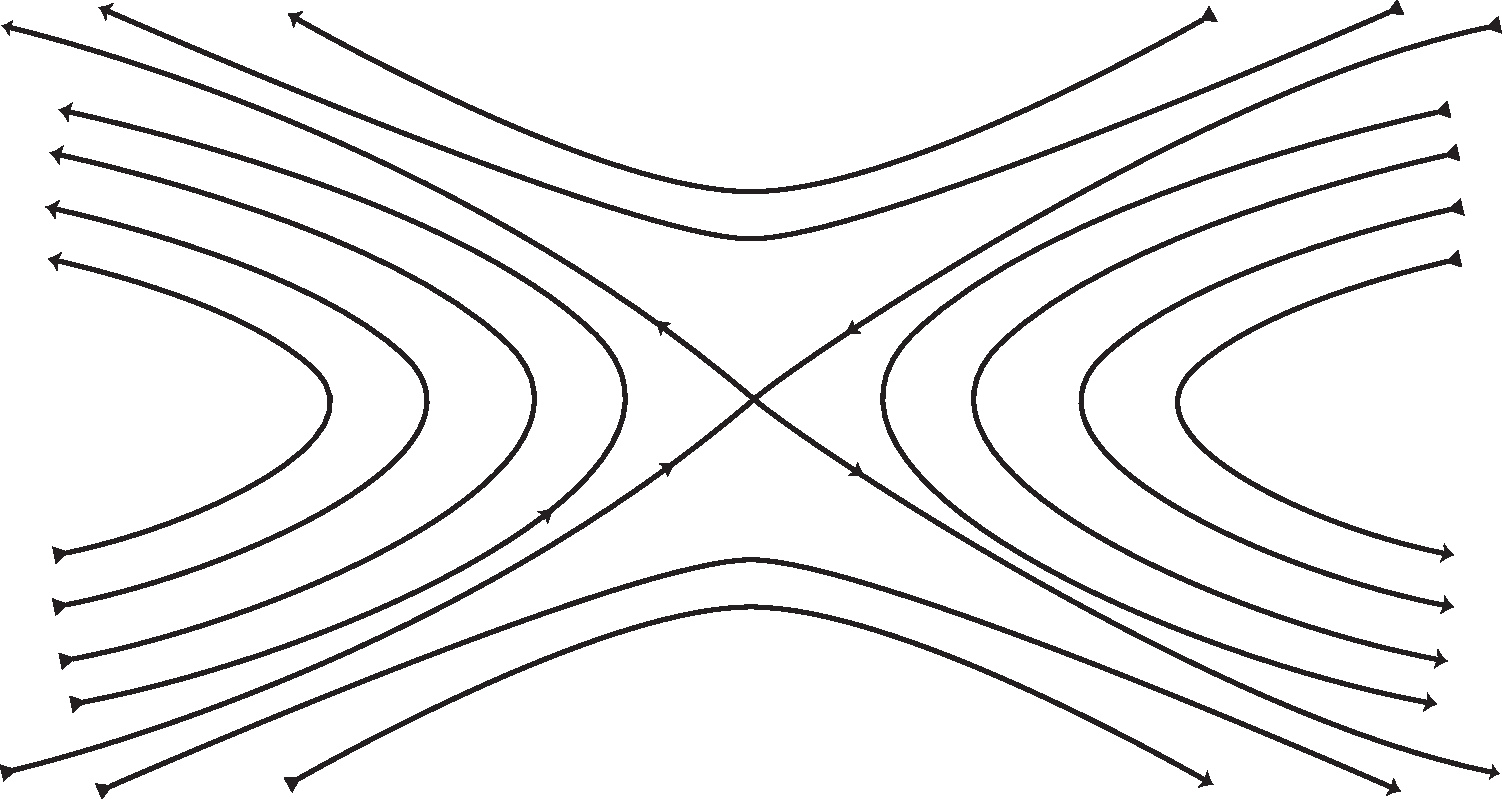
\includegraphics[width=4.5cm]{Graficos/figura19}
	
		\caption{ }
		\label{fig:M-19}
	\end{figure}
\end{observ}

\begin{observ}
Para los casos frontera no mencionados en el teorema \eqref{teo-6}, se tiene:
\begin{APAitemize}
	\item Si el sistema lineal asociado tiene un nodo frontera en \((0,0)\) (caso D), el sistema lineal puede tener
	un nodo o un foco.
	\item Si el sistema lineal asociado tiene un centro en \((0,0)\) (caso E), el sistema no lineal puede tener un
	centro o un foco.
\end{APAitemize}	
\end{observ}

\begin{ejem}
	Sea el sistema
	\[
	\begin{cases}
		\dfrac{dx}{dt}=-y+ax (x^2+y^2)  ,	\vspace{0.3em}
		\\
		\dfrac{dy}{dt}=x+ay(x^2+y^2),
	\end{cases}
	\]
	donde \(a\) es un parámetro. Mostrar que la linealización predice un centro o un foco en el origen. Mostrar que 	realmente corresponde a un foco.
\end{ejem}	
	\begin{proof}[Solución]
		El sistema lineal asociado es:
		\[
		\begin{cases}
		\dfrac{dx}{dt}=-y  ,	\vspace{0.3em}
		\\
		\dfrac{dy}{dt}=x.
	\end{cases}
		\]
		Para este último, \((0,0)\) es un centro, pero para el sistema no lineal es un foco, para mostrar ello, cambiemos el sistema a coordenadas polares. Sea \(x=r\cos\theta\), \(y=r\sin\theta\), \(r^2=x^2+y^2\), luego: \(rr'=xx'+yy'\). De donde:
		\[
		rr'=x\big(-y-ax(x^2+y^2)\big)+y\big(x+ay(x^2+y^2)\big)=ar^4.
		\]
		Por tanto: \(r'=ar^3\).
		
		Como \(\theta=\tan^{-1}(\nicefrac{y}{x})\), se obtiene: \(\theta'=\dfrac{xy'-yx'}{r^2}=1\).
		
		Obteniéndose el sistema en coordenadas polares:
		\[
		\begin{cases}
		r' = a r^3  ,	\vspace{0.3em}
		\\
		\theta' = 1.
		\end{cases}
		\]
		La solución es: \(r=\nicefrac{1}{\sqrt{c-2at}}\), \(\theta=t+t_0\) que corresponde a una familia de espirales.
		
		Luego si \(a<0\) entonces \(\lim_{t\to\infty}r(t)=0\), o sea que el origen es asintóticamente estable (es un sumidero) y si  \(a>0\) entonces \(\lim_{t\to-\infty}r(t)=0\) o sea que el origen es inestable (es una fuente), si \(a=0\) entonces \(r(t)=r_0\) o sea que el origen es un centro (ver figura \ref{fig:M-20}). Obsérvese que \(a=0\) es un punto de bifurcación.	\qedhere
		%
		\vspace{-1\baselineskip}
	\begin{figure}[H]
		\captionsetup{justification=centering, labelfont=footnotesize, font=footnotesize}
		\centering
		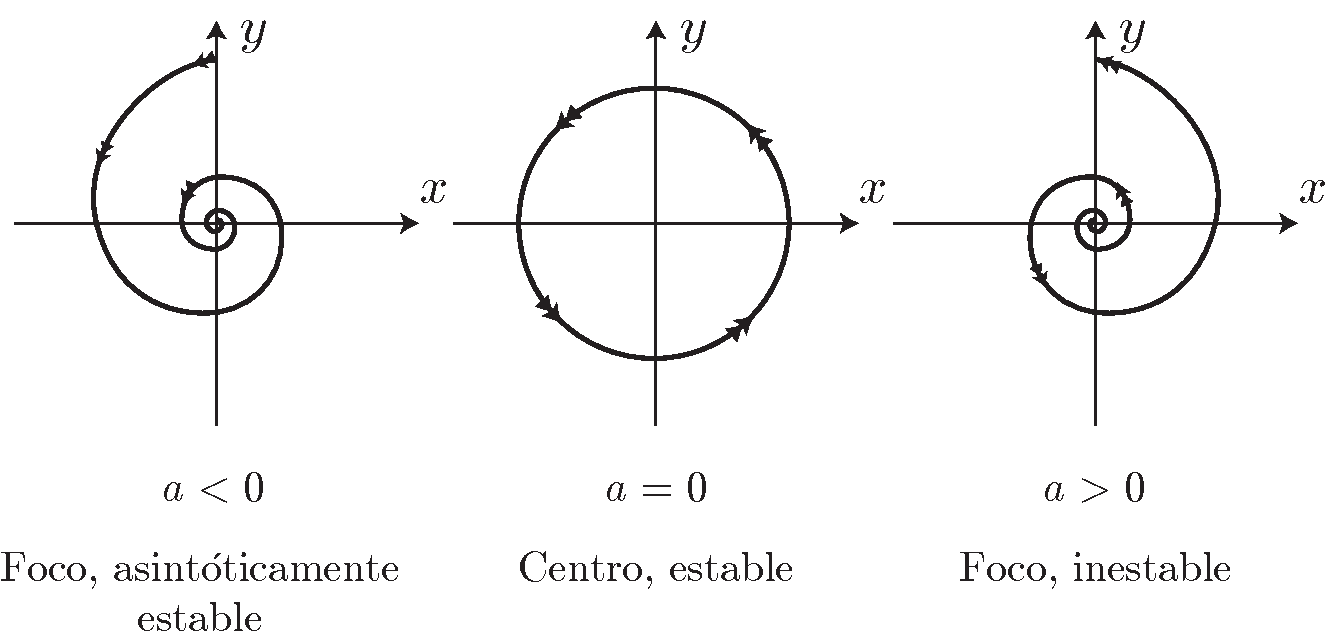
\includegraphics[scale=0.35]{Graficos/figura20}
	
		\caption{ }
		\label{fig:M-20}
	\end{figure}
		%
	\end{proof}


%
\subsubsection{Estabilidad para sistemas no lineales}

\begin{teorema}\label{teo-7}
	Sea \((0,0)\) un punto crítico simple del sistema no lineal \eqref{m-16} y considérese el sistema lineal
	asociado.
	\begin{APAenumerate}
		\item Si el punto crítico \((0,0)\) del sistema lineal es asintóticamente estable, entonces también es asintóticamente estable para el sistema no lineal.
		\item Si el punto crítico\((0,0)\) del sistema lineal asociado es inestable, entonces es inestable para el sistema lineal.
		\item Si el punto crítico \((0,0)\) del sistema lineal asociado es estable pero no asintóticamente estable, entonces para el sistema no lineal puede ser estable, asintóticamente estable o inestable.
	\end{APAenumerate}
\end{teorema}

\begin{observ}
	En el caso 2 del teorema anterior se puede debilitar la hipótesis con la condición
	\begin{equation}\label{m-19}
		\det\begin{pmatrix} a_1 & b_1 \\ a_2 & b_2\end{pmatrix}=0
	\end{equation}
	y dejar las otras condiciones
	\[begin{align*}]
	\lim_{(x,y)\to(0,0)}\dfrac{f(x,y)}{\sqrt{x^2+y^2}}=0 \yds
	\lim_{(x,y)\to(0,0)}\dfrac{g(x,y)}{\sqrt{x^2+y^2}}=0.
	\]
	El resultado también se produce, es decir, si el punto crítico \((0,0)\) del sistema lineal asociado es inestable, entonces también lo es para el sistema no lineal.
\end{observ}


\begin{ejem}
	Sea el sistema:
	\[
	\begin{cases}
		\dfrac{dx}{dt}=-2x+3y+xy ,	\vspace{0.3em}
		\\
		\dfrac{dy}{dt}=-x+y-2xy^2,
	\end{cases}
	\]
	del sistema se puede concluir que 
	\[
		\det\begin{pmatrix} a_1 & b_1 \\ a_2 & b_2 \end{pmatrix}=1\neq 0.
	\]
	Es claro que  \((0,0)\) es un punto crítico simple, en este caso:
	\begin{align*}
		p&=-(a_1+b_2)=-(-2+1)=1>0\\
		q&=a_1b_2-a_2b_1=1>0.
	\end{align*}
	Luego, el punto crítico \((0,0)\) es asintóticamente estable para el sistema lineal y para el sistema no lineal.
\end{ejem}

\begin{ejem}
	La ecuación del movimiento para las oscilaciones forzadas de un péndulo es:
	\[
	\dfrac{d^2x}{dt^2}+\dfrac{c}{m}\dfrac{dx}{dt}+\dfrac{g}{a}\sen x=0,\quad c>0.
	\]
	El sistema no lineal es:
	\[
	\begin{cases}
		\dfrac{dx}{dt}=y ,	\vspace{0.3em}
		\\
		\dfrac{dy}{dt}=-\dfrac{g}{a}\sen x-\dfrac{c}{m}y.
	\end{cases}
	\]
	El cual puede escribirse de la forma
	\[
	\begin{cases}
		\dfrac{dx}{dt}=y ,	\vspace{0.3em}
		\\
		\dfrac{dy}{dt}=-\dfrac{g}{a}x-\dfrac{c}{m}y+\dfrac{g}{a}(x-\sen x).
	\end{cases}
	\]
	Se puede mostrar fácilmente que:
	\[
	\lim_{(x,y)\to(0,0)}\dfrac{x-\sen x}{\sqrt{x^2+y^2}}=0.
	\]
	Como el punto crítico \((0,0)\) es aislado del sistema lineal asociado
	\[
	\begin{cases}
		\dfrac{dx}{dt}=y ,	\vspace{0.3em}
		\\
		\dfrac{dy}{dt}=-\dfrac{g}{a}x-\dfrac{c}{m}y.
	\end{cases}
	\]
	Entonces \((0,0)\) es un punto crítico simple del sistema no lineal, además:
	\begin{align*}
		p&=-(a_1+b_2)=-\left(0-\dfrac{c}{m}\right)=\dfrac{c}{m}>0\\
		q&=a_1b_2-a_2b_1=0\left(-\dfrac{c}{m}\right)-1\left(-\dfrac{g}{a}\right)=\dfrac{g}{a}>0.
	\end{align*}
	Entonces el origen es un punto crítico asintóticamente estable del sistema lineal y también del no lineal. Esto refleja el hecho físico que si un péndulo se perturba ligeramente el movimiento resultante se extinguirá con el tiempo.
\end{ejem}


\begin{ejem}
	Hallar los puntos críticos, determinar su naturaleza y su estabilidad, para el siguiente sistema:
	\[
	\begin{cases}
		\dfrac{dx}{dt}=-2xy=F(x,y) ,	\vspace{0.3em}
		\\
		\dfrac{dy}{dt}=-x+y+xy-y^3=G(x,y).
	\end{cases}
	\]
\end{ejem}
\begin{proof}[Solución]
	La matriz Jacobiana es
	\[
	\begin{pmatrix} \dfrac{\partial F}{\partial x} & \dfrac{\partial F}{\partial y} \\ \dfrac{\partial G}{\partial x} & \dfrac{\partial G}{\partial y} \end{pmatrix}=\begin{pmatrix} -2y & -2x \\ -1+y & 1+x-3y^2 \end{pmatrix}.
	\]
	Para hallar los puntos críticos resolvemos el sistema:
	\[
	F(x,y)=G(x,y)=0.
	\]
	Obteniéndose como puntos críticos a \((0,0)\), \((0,1)\), \((0,-1)\).
	
	\begin{APAitemize}
		\item Para el punto crítico \((0,0)\) se tiene que la matriz Jacobiana es : \(\begin{bmatrix} 0 & 0 \\ -1 & 1 \end{bmatrix}\) y su determinante es  cero.
		
		El sistema lineal asociado es:
		\[
		\begin{cases}
			x' = a_1 x + b_1 y = 0,
			\\
			y' = a_2x+b_2y=-x+y.
		\end{cases}
		\]
		Los valores propios son \(\lambda_1=0\), \(\lambda_2=1\), los vectores propios asociados son \(\begin{pmatrix} 1 \\ 1\end{pmatrix}\), \(\begin{pmatrix} 0 \\ 1 \end{pmatrix}\) y la solución general es \(\begin{pmatrix} x \\ y \end{pmatrix}=\begin{pmatrix} c_1 \\ c_1+c_2e^t \end{pmatrix}\) que es una familia de semirectas paralelas el eje \(Y\) que comienzan en cada punto de la recta \(y = x\) alejándose de ella, por tanto todos los puntos críticos \(( x, x )\) son inestables, en particular \(( 0 , 0 )\) y por la nota anterior, se concluye que el sistema no lineal es inestable en \(( 0 , 0 )\) (ver figura \ref{fig:M-21})
		%
		\vspace{-1\baselineskip}
	\begin{figure}[H]
		\captionsetup{justification=centering, labelfont=footnotesize, font=footnotesize}
		\centering
		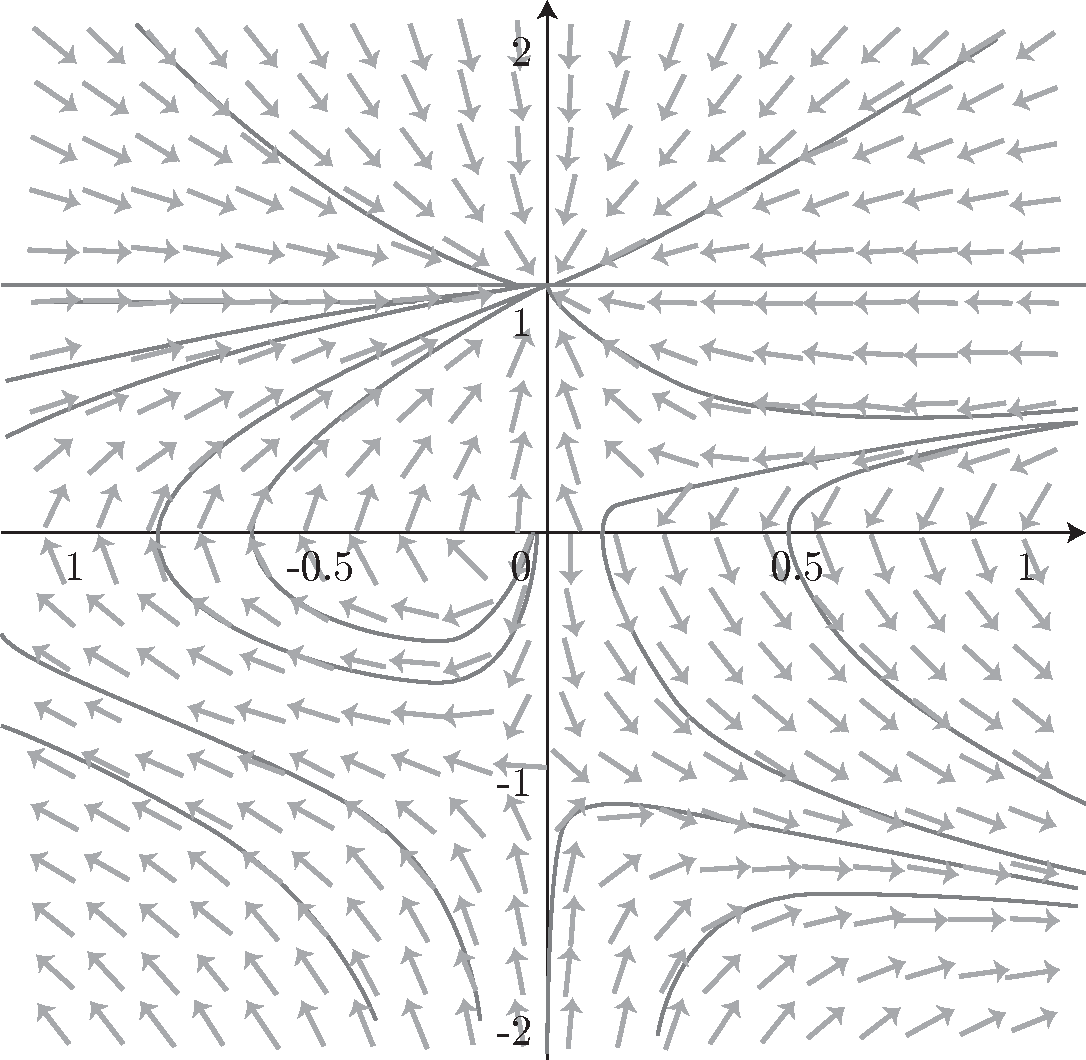
\includegraphics[scale=0.35]{Graficos/figura21}
	
		\caption{ }
		\label{fig:M-21}
	\end{figure}
	
	\item Para el punto \((1,0)\) la matriz Jacobiana es: \(\Big(\begin{smallmatrix} -2 & 0 \\ 0 & -2 \end{smallmatrix} \Big)\) y su determinante es diferente de cero. 
		
		Haciendo \(u=x-x_0=x\), \(v=y-y_0=y-1\), el sistema lineal asociado es:
		\[
		 \begin{pmatrix}u'\\v'\end{pmatrix}=\begin{pmatrix} \dfrac{\partial F}{\partial x} & \dfrac{\partial F}{\partial y} \\ \dfrac{\partial G}{\partial x} & \dfrac{\partial G}{\partial y}\end{pmatrix}\begin{pmatrix} u \\ v\end{pmatrix}=\begin{pmatrix}-2 & 0 \\ 0 & -2 \end{pmatrix}\begin{pmatrix} u \\ v\end{pmatrix}.
		\]
		Los valores propios del sistema lineal asociado son: \(\lambda_{1,2}=-2<0\), por el teorema \eqref{teo-1}, caso D, el punto crítico es un nodo estrella y por el teorema \eqref{teo-2} es asintóticamente estable para el sistema lineal asociado, por la observación del teorema \eqref{teo-6}, referente a los casos frontera y por el teorema \eqref{teo-7} es un nodo o un foco asintóticamente estable.
		
		
	\item Para el punto \((0,-1)\) la matriz Jacobiana es: \(\Big(\begin{smallmatrix} 2 & 0 \\ -2 & -2\end{smallmatrix}\Big)\) y su determinante es diferente de cero. Haciendo \(u=x-x_0=x\),  \(v=y-y_0=y+1\), el sistema lineal asociado es
		\[
		\begin{pmatrix}u'\\v'\end{pmatrix}=\begin{pmatrix} \dfrac{\partial F}{\partial x} & \dfrac{\partial F}{\partial y} \\ \dfrac{\partial G}{\partial x} & \dfrac{\partial G}{\partial y}\end{pmatrix}\begin{pmatrix} u \\ v\end{pmatrix}=\begin{pmatrix} 2 & 0 \\ -2 & -2\end{pmatrix}\begin{pmatrix} u \\ v\end{pmatrix}.
		\]
		Los valores propios  del sistema lineal asociado son: \(\lambda_1=2\), \(\lambda_2=-2\), por el teorema \eqref{teo-1}, el caso B, punto crítico es un punto silla y por el teorema \eqref{teo-2} es inestable para el sistema lineal asociado; entonces para el sistema no lineal, por el teorema \eqref{teo-6} y por el teorema \eqref{teo-7},	\((0,-1)\) es un punto silla inestable.	\qedhere
	\end{APAitemize}
\end{proof}


\begin{ejem}[Dos especies en competencia]
	Supóngase que dos especies liebres y ovejas compiten por el mismo tipo de alimento (grama) y esta cantidad de alimento es limitada, ignorando otros factores como depredadores, factores climáticos, otras fuentes de alimento. Las ecuaciones que modelan este fenómeno son las ecuaciones de Lotka--Volterra
	\[
	\begin{cases}
		x'=x(3-x-2y)=F(x,y),
		\\
		y'=y(2-x-y)=G(x,y),
	\end{cases}
	\]
	donde \(x(t)\) es la población de liebres y \(y(t)\) es la población de ovejas. Hallar los puntos críticos, definir el tipo y estabilidad.
\end{ejem}
\begin{proof}[Solución]
		Los puntos críticos son: \(A(0,0)\), \(B(0,2)\), \(C(3,0)\), \(D(1,1)\).
		
		El Jacobiano es: 
		\[
		J = \begin{pmatrix}\dfrac{\partial F}{\partial x} & \dfrac{\partial F}{\partial y} \\ \dfrac{\partial G}{\partial x} & \dfrac{\partial G}{\partial y} \end{pmatrix}=\begin{pmatrix} 3-2x-y & -2y \\ -y &  2-x-2y\end{pmatrix}.
		\]
		
		\begin{APAenumerate}
			\item Para el punto \(A(0,0)\), \(J=\Big(\begin{smallmatrix}  3 & 0 \\ 0 & 2\end{smallmatrix}\Big) \) y sus valores propios son: \(\lambda_1=3\), \(\lambda_2=2\), luego, \((0,0)\) es un nodo inestable, es decir las trayectorias salen tangencialmente del origen paralelas al vector propio \(v=\begin{pmatrix} 0 \\ 1\end{pmatrix}\) asociado al valor propio \(\lambda_2=2\).
			
			\item Para el punto \(B(0,2)\), \(J=\Big(\begin{smallmatrix}  -1 & 0 \\ -2 & 2 \end{smallmatrix}\Big) \) y sus valores propios son: \(\lambda_1=-1\), \(\lambda_2=2\), luego, \((0,2)\) es un nodo asintóticamente estable, las trayectorias entran al punto crítico en la dirección del vector propio \(v=\begin{pmatrix} 1 \\ -2\end{pmatrix}\) asociado al valor propio \(\lambda_1=-1\).
			
			\item Para el punto \(C(3,0)\), \(J=\Big(\begin{smallmatrix}  -3 & -6 \\ 0 & -1 \end{smallmatrix}\Big) \) y sus valores propios son: \(\lambda_1=-3\), \(\lambda_2=-1\), luego, \((3,0)\) es un nodo asintóticamente estable, las trayectorias entran al punto crítico en la dirección del vector propio \(v=\begin{pmatrix} 3 \\ -1\end{pmatrix}\) asociado al valor propio \(\lambda_1=-1\).
			
			\item Para el punto \(D(1,1)\), \(J=\Big(\begin{smallmatrix} -1 & -2 \\ -1 & -1 \end{smallmatrix}\Big) \) y sus valores propios son: \(\lambda_{1,2}=-1\pm\sqrt{2}\), luego, \((1,1)\) es un punto de silla y como \(p=-(a_1+a_2)=2\) y \(\det A=\left|\begin{smallmatrix} -1 & -2 \\ -1 & -1 \end{smallmatrix}\right|=-1<0\), entonces se tiene que \((1,1)\) es inestable.
		\end{APAenumerate}
	
	
	El retrato de fase mostrado en la figura \ref{fig:M-22} tiene la siguiente interpretación biológica: una de las dos especies 	inevitablemente se extingue, por ejemplo, por debajo de la curva l las trayectorias tienden al punto crítico \(C(3,0)\) lo cual quiere decir que las ovejas se extinguen; cuando las trayectorias están encima de la curva \(l\) las trayectorias tienden al punto crítico \(B(0,2)\) lo cual quiere decir que se extinguen las liebres.
	
	
	\end{proof}
	\newpage
%
	
	\begin{figure}[H]
		\captionsetup{justification=centering, labelfont=footnotesize, font=footnotesize}
		\centering
		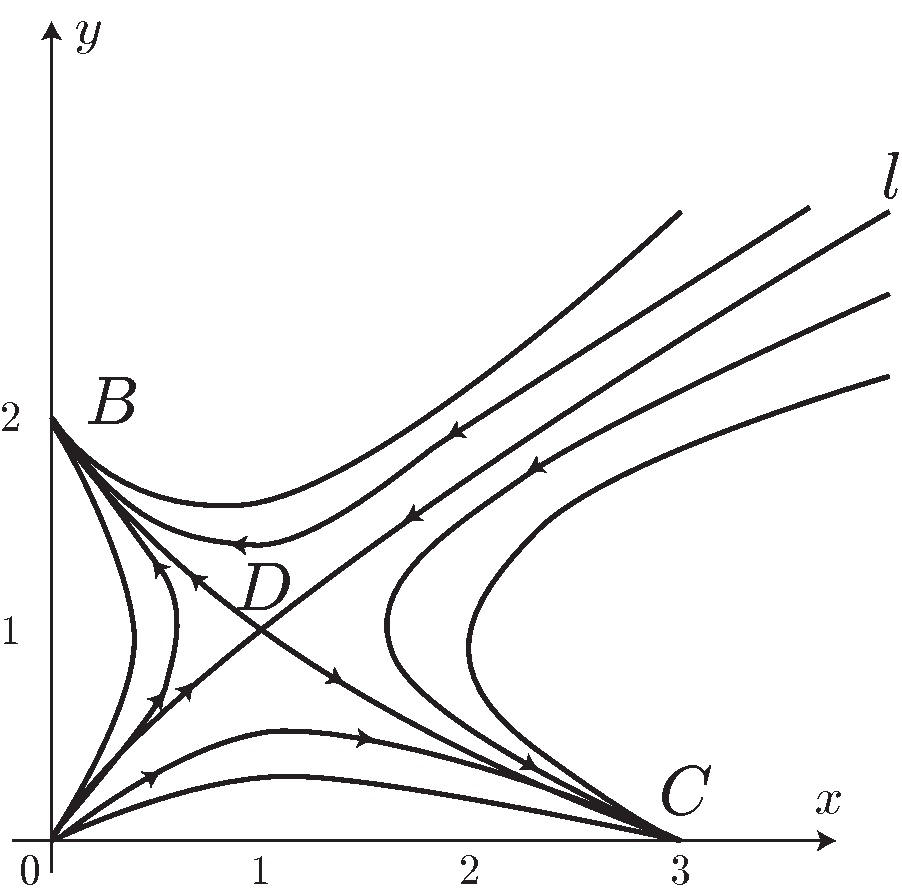
\includegraphics[width=4.5cm]{Graficos/figura22}
	
		\caption{ }
		\label{fig:M-22}
	\end{figure}


\begin{ejem}[Dos especies: un depredador y una presa]
	Sea \(x(t)\) el número de presas (por ejemplo liebres) y \(y(t)\) el número de depredadores (por ejemplo lobos). A principios del siglo XX el matemático italiano Vito Volterra modeló este problema, haciendo las siguientes caracterizaciones:
	\begin{APAitemize}
		\item En ausencia de depredadores, la población de presas crece a la tasa natural \(\nicefrac{dx}{dt}=ax\), \(a>0\)
		\item En ausencia de presas, la población depredadora decrece a la tasa natural \(\nicefrac{dy}{dt}=-cy\), \(c>0\)
		\item Cuando las presas y los depredadores cohabitan el mismo lugar, las tasa naturales de crecimiento y   decrecimiento de presas y depredadores respectivamente son proporcionales al número de encuentros de ambos, es decir, son proporcionales a \(xy\). En consecuencia, el efecto de que los depredadores devoren a sus presas, produce una tasa decreciente de interacción \(-bxy\) con respecto a la población de presas \(x(t)\) y una tasa creciente \(dxy\) con respecto a la población de depredadores \(y(t)\).
		
		En consecuencia, sumando las tasan naturales y las tasa de interacción, se tienen las ecuaciones para una especie depredadora y una especie presa:
		\[
		\begin{cases}
		\dfrac{dx}{dt}=ax-bxy=x(a-by)  ,	\vspace{0.3em}
		\\
		\dfrac{dy}{dt}=-cy+dxy=y(-c+dx).
	\end{cases}
		\]
		Haciendo la consideración adicional de que en ausencia de depredadores el crecimiento de las presas es
		logístico, es decir, es directamente proporcional a su población como también a la diferencia con su población máxima y tomando \(a=b=c=d=1\), se tiene el sistema:
		\[
		\begin{cases}
		\dfrac{dx}{dt}=x-xy+\varepsilon x(1-x),	\vspace{0.3em}
		\\
		\dfrac{dy}{dt}=-y+xy.
	\end{cases}
		\]
	\end{APAitemize}
	Analizar la estabilidad, variando el parámetro \(\varepsilon\), para \(\varepsilon\geq 0\).
\end{ejem}
\begin{proof}[Solución]
		Los puntos críticos son \((0,0)\) y \((1,1)\). El Jacobiano es:
		\[
			J=\begin{pmatrix} \dfrac{\partial F}{\partial x} & \dfrac{\partial F}{\partial y} \\ \dfrac{\partial G}{\partial x} & \dfrac{\partial G}{\partial x}\end{pmatrix}=\begin{pmatrix} 1-y+\varepsilon(1-2x) & -x \\ y & -1+x\end{pmatrix}.
		\]
		Para \(\varepsilon=0\) tenemos (ver figura \ref{fig:M-23}):
		%
		\vspace{-1\baselineskip}
	\begin{figure}[H]
		\captionsetup{justification=centering, labelfont=footnotesize, font=footnotesize}
		\centering
		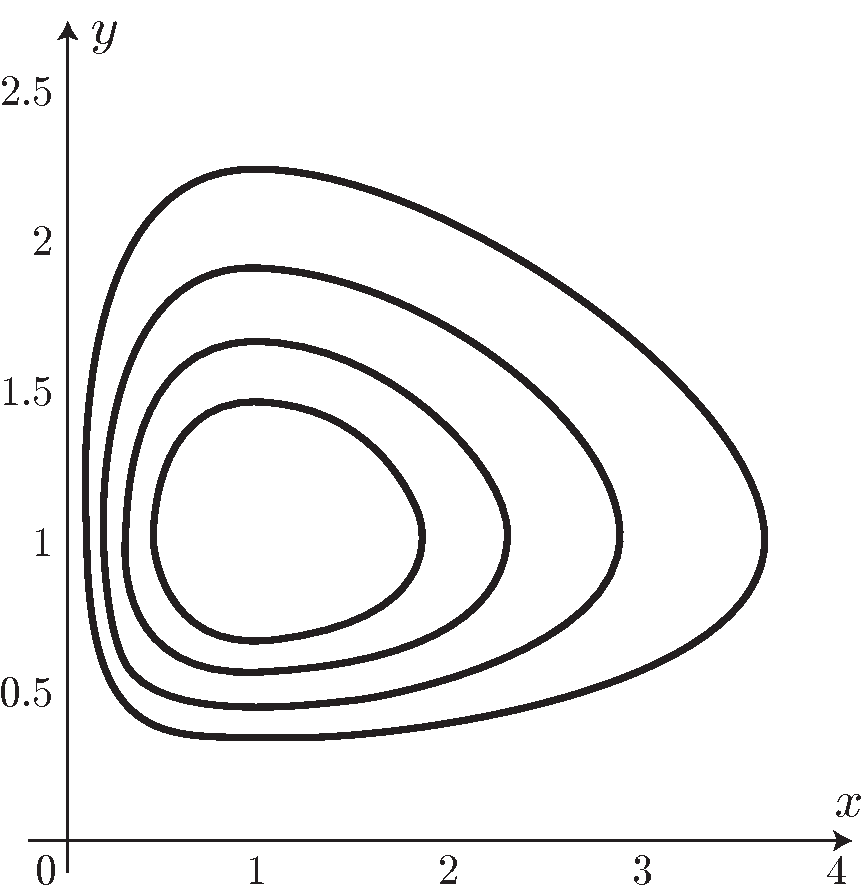
\includegraphics[width=4.5cm]{Graficos/figura23}
	
		\caption{Sistema depredador-presa, \(\varepsilon=0\)}
		\label{fig:M-23}
	\end{figure}
	
	\begin{APAenumerate}
			\item Para el punto crítico \((0,0)\), \(J= \Big(\begin{smallmatrix} 1 & 0 \\ 0 & -1\end{smallmatrix} \Big)\) y sus valores propios son: \(\lambda_1=1\), \(\lambda_2=1\), luego \((0,0)\) es un punto de silla estable.
			\item Para el punto crítico \((1,1)\), \(J= \Big(\begin{smallmatrix} 0 & -1 \\ 1 & 0 \end{smallmatrix}\Big) \) y sus valores propios son: \(\lambda_1=i\), \(\lambda_2=-i\), luego \((1,1)\) es un centro estable, las trayectorias giran alrededor el punto crítico.
		\end{APAenumerate}
	
	\vspace{1\baselineskip}
	Para \(0<\varepsilon<2\) tenemos (ver figura \ref{fig:M-24}):
	%
		%\vspace{-1\baselineskip}
	\begin{figure}[H]
		\captionsetup{justification=centering, labelfont=footnotesize, font=footnotesize}
		\centering
		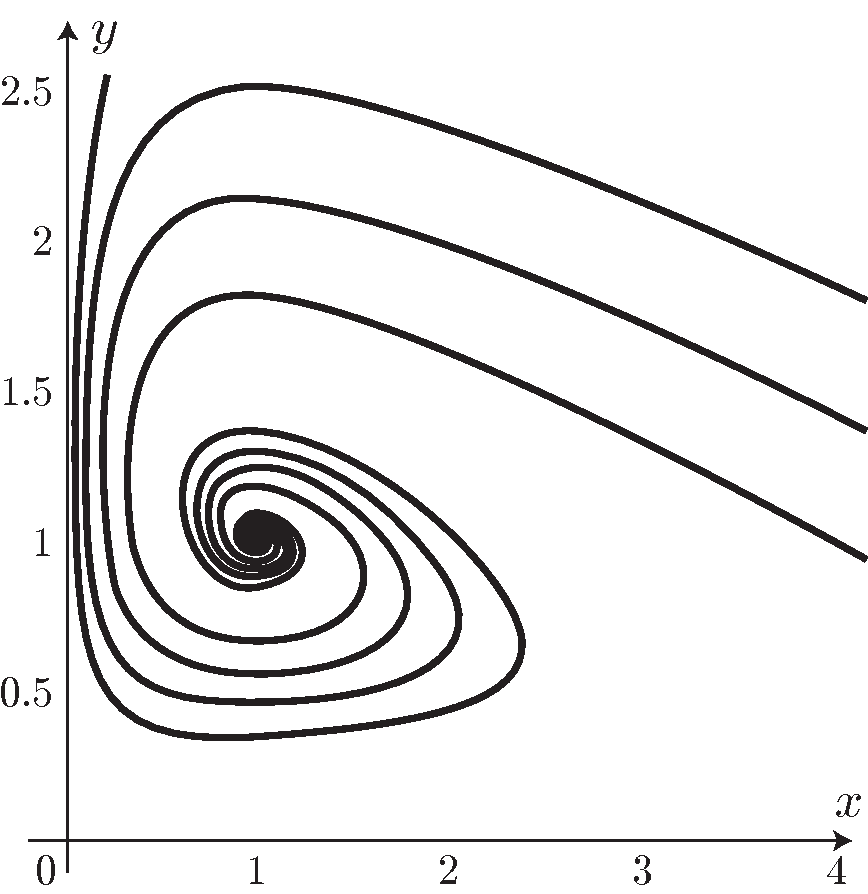
\includegraphics[width=4.5cm]{Graficos/figura24}
	
		\caption{Sistema depredador-presa, \(\varepsilon \in (0,2)\)}
		\label{fig:M-24}
	\end{figure}

	\begin{APAenumerate}
		\item Para el punto crítico \((0,0)\), \(J= \Big(\begin{smallmatrix}  1+\varepsilon & 0 \\ 0 & -1 \end{smallmatrix} \Big) \) y sus valores propios son: \(\lambda_1=1+\varepsilon>0\), \(\lambda_2=-1\), luego \((0,0)\) es un punto de silla inestable.
		\item Para el punto crítico \((1,1)\), \(J= \Big(\begin{smallmatrix}  -\varepsilon & -1 \\ 1 & 0\end{smallmatrix} \Big) \) y sus valores propios son: \(\lambda_{1,2}=\dfrac{-\varepsilon\pm\sqrt{4-\varepsilon^2}i}{2}\), luego \((1,1)\) es un foco asintóticamente estable.
	\end{APAenumerate}

	\newpage
	Para \(\varepsilon=2\) tenemos (ver figura \ref{fig:M-25}):
	
	\begin{figure}[H]
		\captionsetup{justification=centering, labelfont=footnotesize, font=footnotesize}
		\centering
		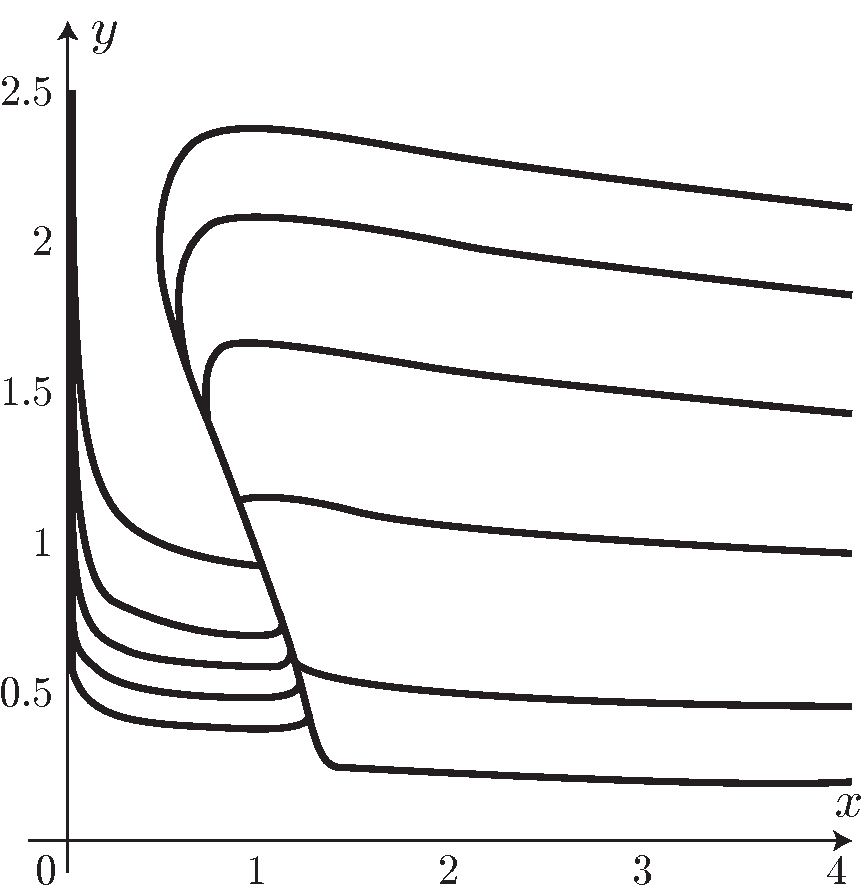
\includegraphics[width=4.5cm]{Graficos/figura25}
	
		\caption{Sistema depredador-presa, \(\varepsilon=2\)}
		\label{fig:M-25}
	\end{figure}
	
	\begin{APAenumerate}
	\item Para el punto crítico \((0,0)\), \(J= \Big(\begin{smallmatrix}  3 & 0 \\ 0 & -1 \end{smallmatrix} \Big) \) y sus valores propios son: \(\lambda_1=-1\), \(\lambda_2=3\), luego \((0,0)\)  es un punto de silla inestable.
	\item Para el punto crítico \((1,1)\), \(J= \Big(\begin{smallmatrix}  -2 & -1 \\ 1 & 0 \end{smallmatrix} \Big) \) y sus valores propios son: \(\lambda_{1,2}=-1\), luego \((1,1)\) es un nodo o un foco asintóticamente estable.
\end{APAenumerate}


	Para \(\varepsilon>2\) tenemos (ver figura \ref{fig:M-26}):
	
	\begin{figure}[H]
		\captionsetup{justification=centering, labelfont=footnotesize, font=footnotesize}
		\centering
		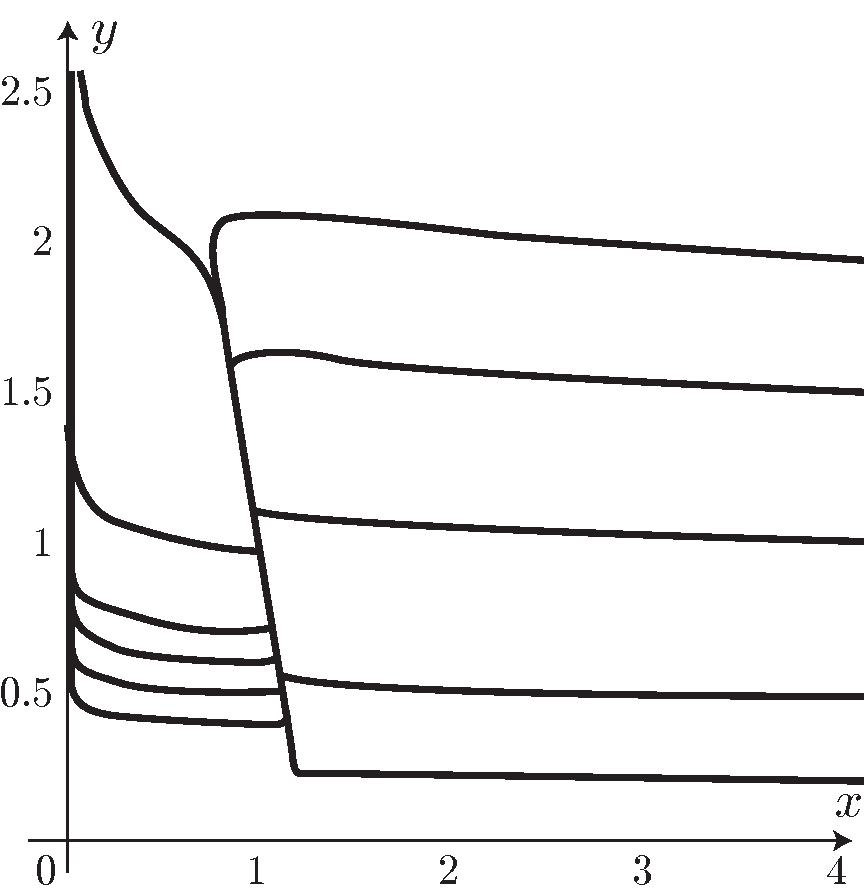
\includegraphics[width=4.5cm]{Graficos/figura26}
	
		\caption{Sistema depredador-presa, \(\varepsilon>2\)}
		\label{fig:M-26}
	\end{figure}

	\begin{APAenumerate}
	\item Para el punto crítico \((0,0)\), \(J= \Big(\begin{smallmatrix}  1+\varepsilon & 0 \\ 0 & -1 \end{smallmatrix} \Big) \) y sus valores propios son: \(\lambda_1=\varepsilon+1\), \(\lambda_2=-1\), luego \((0,0)\) es un punto de silla inestable.
	\item Para el punto crítico \((1,1)\), \(J= \Big(\begin{smallmatrix}   -\varepsilon & -1 \\ 1 & 0 \end{smallmatrix} \Big) \) y sus valores propios son: \(\lambda_{1,2}=\dfrac{-\varepsilon\pm\sqrt{\varepsilon^2-4}}{2}<0\), luego \((1,1)\) es un nudo asintóticamente estable.
\end{APAenumerate}


Obsérvese que para soluciones para \(\varepsilon=0\) las soluciones son estructuralmente (son estables y periódicas) distintas de las \(\varepsilon>0\) (asintóticamente estables y no periódica, por este cambio estructural en las soluciones, se dice que en \(\varepsilon=0\) se produce una bifurcación.
\end{proof}









\nocite{bib-M}

}







\end{document}































